%% (Master) Thesis template
% Template version used: v1.4
%
% Largely adapted from Adrian Nievergelt's template for the ADPS
% (lecture notes) project.


%% We use the memoir class because it offers a many easy to use features.
\documentclass[11pt,a4paper,titlepage]{memoir}

%% Packages
%% ========

%% LaTeX Font encoding -- DO NOT CHANGE
\usepackage[OT1]{fontenc}

%% Babel provides support for languages.  'english' uses British
%% English hyphenation and text snippets like "Figure" and
%% "Theorem". Use the option 'ngerman' if your document is in German.
%% Use 'american' for American English.  Note that if you change this,
%% the next LaTeX run may show spurious errors.  Simply run it again.
%% If they persist, remove the .aux file and try again.
\usepackage[english]{babel}

%% Input encoding 'utf8'. In some cases you might need 'utf8x' for
%% extra symbols. Not all editors, especially on Windows, are UTF-8
%% capable, so you may want to use 'latin1' instead.
\usepackage[utf8]{inputenc}

%% This changes default fonts for both text and math mode to use Herman Zapfs
%% excellent Palatino font.  Do not change this.
\usepackage[sc]{mathpazo}

%% The AMS-LaTeX extensions for mathematical typesetting.  Do not
%% remove.
\usepackage{amsmath,amssymb,amsfonts,mathrsfs}

%% NTheorem is a reimplementation of the AMS Theorem package. This
%% will allow us to typeset theorems like examples, proofs and
%% similar.  Do not remove.
%% NOTE: Must be loaded AFTER amsmath, or the \qed placement will
%% break
\usepackage[amsmath,thmmarks]{ntheorem}

%% LaTeX' own graphics handling
\usepackage{graphicx}

%% We unfortunately need this for the Rules chapter.  Remove it
%% afterwards; or at least NEVER use its underlining features.
\usepackage{soul}

%% This allows you to add .pdf files. It is used to add the
%% declaration of originality.
\usepackage{pdfpages}

%% Some more packages that you may want to use.  Have a look at the
%% file, and consult the package docs for each.
%% See the TeXed file for more explanations

%% [OPT] Multi-rowed cells in tabulars
%\usepackage{multirow}

%% [REC] Intelligent cross reference package. This allows for nice
%% combined references that include the reference and a hint to where
%% to look for it.
\usepackage{varioref}

%% [OPT] Easily changeable quotes with \enquote{Text}
%\usepackage[german=swiss]{csquotes}

%% [REC] Format dates and time depending on locale
\usepackage{datetime}

%% [OPT] Provides a \cancel{} command to stroke through mathematics.
%\usepackage{cancel}

%% [NEED] This allows for additional typesetting tools in mathmode.
%% See its excellent documentation.
\usepackage{mathtools}

%% [ADV] Conditional commands
%\usepackage{ifthen}

%% [OPT] Manual large braces or other delimiters.
%\usepackage{bigdelim, bigstrut}

%% [REC] Alternate vector arrows. Use the command \vv{} to get scaled
%% vector arrows.
\usepackage[h]{esvect}

%% [NEED] Some extensions to tabulars and array environments.
\usepackage{array}

%% [OPT] Postscript support via pstricks graphics package. Very
%% diverse applications.
%\usepackage{pstricks,pst-all}

%% [?] This seems to allow us to define some additional counters.
%\usepackage{etex}

%% [ADV] XY-Pic to typeset some matrix-style graphics
%\usepackage[all]{xy}

%% [OPT] This is needed to generate an index at the end of the
%% document.
%\usepackage{makeidx}

%% [OPT] Fancy package for source code listings.  The template text
%% needs it for some LaTeX snippets; remove/adapt the \lstset when you
%% remove the template content.
\usepackage{listings}
\lstset{language=TeX,basicstyle={\normalfont\ttfamily}}

%% [REC] Fancy character protrusion.  Must be loaded after all fonts.
\usepackage[activate]{pdfcprot}

%% [REC] Nicer tables.  Read the excellent documentation.
\usepackage{booktabs}

\usepackage{tcolorbox}

%% Our layout configuration.  DO NOT CHANGE.
%% Memoir layout setup

%% NOTE: You are strongly advised not to change any of them unless you
%% know what you are doing.  These settings strongly interact in the
%% final look of the document.

% Dependencies
\usepackage{ETHlogo}

% Turn extra space before chapter headings off.
\setlength{\beforechapskip}{0pt}

\nonzeroparskip
\parindent=0pt
\defaultlists

% Chapter style redefinition
\makeatletter

\if@twoside
  \pagestyle{Ruled}
  \copypagestyle{chapter}{Ruled}
\else
  \pagestyle{ruled}
  \copypagestyle{chapter}{ruled}
\fi
\makeoddhead{chapter}{}{}{}
\makeevenhead{chapter}{}{}{}
\makeheadrule{chapter}{\textwidth}{0pt}
\copypagestyle{abstract}{empty}

\makechapterstyle{bianchimod}{%
  \chapterstyle{default}
  \renewcommand*{\chapnamefont}{\normalfont\Large\sffamily}
  \renewcommand*{\chapnumfont}{\normalfont\Large\sffamily}
  \renewcommand*{\printchaptername}{%
    \chapnamefont\centering\@chapapp}
  \renewcommand*{\printchapternum}{\chapnumfont {\thechapter}}
  \renewcommand*{\chaptitlefont}{\normalfont\huge\sffamily}
  \renewcommand*{\printchaptertitle}[1]{%
    \hrule\vskip\onelineskip \centering \chaptitlefont\textbf{\vphantom{gyM}##1}\par}
  \renewcommand*{\afterchaptertitle}{\vskip\onelineskip \hrule\vskip
    \afterchapskip}
  \renewcommand*{\printchapternonum}{%
    \vphantom{\chapnumfont {9}}\afterchapternum}}

% Use the newly defined style
\chapterstyle{bianchimod}

\setsecheadstyle{\Large\bfseries\sffamily}
\setsubsecheadstyle{\large\bfseries\sffamily}
\setsubsubsecheadstyle{\bfseries\sffamily}
\setparaheadstyle{\normalsize\bfseries\sffamily}
\setsubparaheadstyle{\normalsize\itshape\sffamily}
\setsubparaindent{0pt}

% Set captions to a more separated style for clearness
\captionnamefont{\sffamily\bfseries\footnotesize}
\captiontitlefont{\sffamily\footnotesize}
\setlength{\intextsep}{16pt}
\setlength{\belowcaptionskip}{1pt}

% Set section and TOC numbering depth to subsection
\setsecnumdepth{subsection}
\settocdepth{subsection}

%% Titlepage adjustments
\pretitle{\vspace{0pt plus 0.7fill}\begin{center}\HUGE\sffamily\bfseries}
\posttitle{\end{center}\par}
\preauthor{\par\begin{center}\let\and\\\Large\sffamily}
\postauthor{\end{center}}
\predate{\par\begin{center}\Large\sffamily}
\postdate{\end{center}}

\def\@advisors{}
\newcommand{\advisors}[1]{\def\@advisors{#1}}
\def\@department{}
\newcommand{\department}[1]{\def\@department{#1}}
\def\@thesistype{}
\newcommand{\thesistype}[1]{\def\@thesistype{#1}}

\renewcommand{\maketitlehooka}{\noindent\ETHlogo[2in]}

\renewcommand{\maketitlehookb}{\vspace{1in}%
  \par\begin{center}\Large\sffamily\@thesistype\end{center}}

\renewcommand{\maketitlehookd}{%
  \vfill\par
  \begin{flushright}
    \sffamily
    \@advisors\par
    \@department, UVigo \& UdC
  \end{flushright}
}

\checkandfixthelayout

\setlength{\droptitle}{-48pt}

\makeatother

% This defines how theorems should look. Best leave as is.
\theoremstyle{plain}
\setlength\theorempostskipamount{0pt}

%%% Local Variables:
%%% mode: latex
%%% TeX-master: "thesis"
%%% End:


%% Theorem environments.  You will have to adapt this for a German
%% thesis.
%% Theorem-like environments

%% This can be changed according to language. You can comment out the ones you
%% don't need.

\numberwithin{equation}{chapter}

%% German theorems
%\newtheorem{satz}{Satz}[chapter]
%\newtheorem{beispiel}[satz]{Beispiel}
%\newtheorem{bemerkung}[satz]{Bemerkung}
%\newtheorem{korrolar}[satz]{Korrolar}
%\newtheorem{definition}[satz]{Definition}
%\newtheorem{lemma}[satz]{Lemma}
%\newtheorem{proposition}[satz]{Proposition}

%% English variants
\newtheorem{theorem}{Theorem}[chapter]
\newtheorem{example}[theorem]{Example}
\newtheorem{remark}[theorem]{Remark}
\newtheorem{corollary}[theorem]{Corollary}
\newtheorem{definition}[theorem]{Definition}
\newtheorem{lemma}[theorem]{Lemma}
\newtheorem{proposition}[theorem]{Proposition}

%% Proof environment with a small square as a "qed" symbol
\theoremstyle{nonumberplain}
\theorembodyfont{\normalfont}
\theoremsymbol{\ensuremath{\square}}
\newtheorem{proof}{Proof}
%\newtheorem{beweis}{Beweis}


%% Helpful macros.
%% Custom commands
%% ===============

%% Special characters for number sets, e.g. real or complex numbers.
\newcommand{\C}{\mathbb{C}}
\newcommand{\K}{\mathbb{K}}
\newcommand{\N}{\mathbb{N}}
\newcommand{\Q}{\mathbb{Q}}
\newcommand{\R}{\mathbb{R}}
\newcommand{\Z}{\mathbb{Z}}
\newcommand{\X}{\mathbb{X}}

%% Fixed/scaling delimiter examples (see mathtools documentation)
\DeclarePairedDelimiter\abs{\lvert}{\rvert}
\DeclarePairedDelimiter\norm{\lVert}{\rVert}

%% Use the alternative epsilon per default and define the old one as \oldepsilon
\let\oldepsilon\epsilon
\renewcommand{\epsilon}{\ensuremath\varepsilon}

%% Also set the alternate phi as default.
\let\oldphi\phi
\renewcommand{\phi}{\ensuremath{\varphi}}


%% Make document internal hyperlinks wherever possible. (TOC, references)
%% This MUST be loaded after varioref, which is loaded in 'extrapackages'
%% above.  We just load it last to be safe.
\usepackage[linkcolor=black,colorlinks=true,citecolor=black,filecolor=black]{hyperref}


%% Document information
%% ====================

\title{Confidentiality and trace in malware samples}
\author{David Álvarez Pérez}
\thesistype{Master Thesis}
\advisors{Advisors: Manuel Fernández Veiga}
\department{Máster Interuniversitario en Ciberseguridad}
\date{January 19, 2020}

\begin{document}

\frontmatter

%% Title page is autogenerated from document information above.  DO
%% NOT CHANGE.
\begin{titlingpage}
  \calccentering{\unitlength}
  \begin{adjustwidth*}{\unitlength-24pt}{-\unitlength-24pt}
    \maketitle
  \end{adjustwidth*}
\end{titlingpage}

%% The abstract of your thesis.  Edit the file as needed.
\begin{abstract}
  Malware sample confidentiality is an unsolved problem which affects the
  major security products including antiviruses, threat hunting and threat
  intelligence products\cite{EuropeanParliamentReportOnCyberDefence}\cite{EuropeanParliamentDesignatingAsDangerous} which, always, in greater or lesser volume,
  potentially collect confidential elements\cite{Kaspersky2020EulaEn}\cite{McAfeeEnterpriseEulaEnGb}\cite{MalwarebytesEula} (including files, system events,
  network traffic because of firewall capabilities, etc.). These are not
  necessary malware, but are also paradoxically called malware samples. This
  happens because new knowledge cannot come but from other place than unknown
  and undetected elements. We consider this a critical issue because the
  capabilities of surveillance of free and paid security products (including
  those that come built-in the operating system) are huge\cite{KasperskyBoundariesOfTrust} and growing\cite{ThreatHuntingForDummies}\cite{ProactiveHunting} in terms
  of local system and local area network access.  The solution proposed in
  this work to this confidentiality risk and access logging problem involves
  the design of a new encrypted malware sample format: Universal Malware
  Sample Encryption (UMSE).  UMSE is a rich format. It can represent: software
  threats, hardware threats\cite{HardwareMalware}, the mixing of both and takes into account very
  important forgotten aspects like: potential malicious elements context\cite{ContextBasedMalware}\cite{LearningFromContext}, life
  cycle\cite{SoftwareEngineering} and variety of nature of the elements (not limited to files\cite{ResidentViruses}\cite{FilelessAttacks}\cite{AdvacedVolatileThreat}) and some
  other things which finally improve the sample quality acquisition, storage
  and transport positively impacting all subsequent reverse engineering tasks
  and users confidentiality.
\end{abstract}


%% TOC with the proper setup, do not change.
\cleartorecto
\tableofcontents
\mainmatter

%% Your real content!
% Some commands used in this file
\newcommand{\package}{\emph}

\chapter{Introduction}

Understanding by malware sample the evidence set of any kind of malicious
element, hardware and/or software, in a vital cycle state and belonging a
context, the present work addresses the malware sample process: acquisition,
efficient storage, confidentiality and access logging problem.

The result of this work is an encrypted malware sample format called Universal
Malware Sample Encryption (hereafter, UMSE). The development, far from being
limited to the sheer format specification, consisted in the following:
\begin{itemize}
\item UMSE format documentation and specification.
\item A Microsoft Windows Portable Executable\cite{MicrosoftPecoff} dynamic linking library\cite{DynamicLinkLibraries}
  implementing all necessary functions to work with UMSE, for instance:
  generate an UMSE malware sample, decrypt some sample parts regarding
  individual parts confidentiality, etc.  This library was developed in C/C++
  to be used by security products which are mostly developed in these
  languages (well, although it can be called from other languages).
\item A very elementary antimalware agent simulator which acquires system
  elements demonstrating how easy is to integrate the UMSE dynamic linking
  library with existing security products.
\item An intelligence tool. It consists in a web panel allowing to operate and
  manage UMSE malware samples stored in a generic database. All malware
  samples come from the mentioned antimalware agent simulator, which
  recollects potential malicious elements and sends them to this server. On
  the other hand, by virtue of UMSE format, each operation over the samples
  can be logged, as is this case here.
\item A Shell, allowing the malware analyst to communicate with the
  intelligence tool to work with samples. Possible operations are some of
  which, at least two, deserve mention: UMSE sample downloading and UMSE
  sample parts decryption in case that the analyst was sufficiently privileged
  in comparison to, not only the global, but also the confidentiality level
  for the specific individual sample parts.
\item A tool to quickly and easily generate samples, useful when encryption is
  not a must.
\end{itemize}
Below is the status of current malware sample acquisition, storage and
confidentiality in order to show the problem addressed in the rest of this
work.

% Structure of the document.
\chapter{Malware and malware samples}

First of all, before addressing the question of what a ``malware sample'' is,
let us analyze what a ``malware'' is.

The National Institute of Standards and Technologies (NIST) throws the
following definition of malware: ``Software or firmware intended to perform an
unauthorized process that will have adverse impact on the confidentiality,
integrity, or availability of an information system. A virus, worm, Trojan
horse, or other code-based entity that infects a host. Spyware and some forms
of adware are also examples of malicious
code.''\cite{Nist2013}

And RFC4949\cite{Rfc4949} defines
``malicious logic'' as ``Hardware, firmware, or software that is intentionally
included or inserted in a system for a harmful purpose.''

A lot of definitions of ``malware'' do
exist\cite{NistGlossary2020} but in this work we propose to use this one to remark some key points of
malware nature:
\begin{tcolorbox}
  Any element, hardware, software and/or firmware, determined malicious in
  some context and in a state of its life cycle.
\end{tcolorbox}

Notice that proposed malware definition has a strong subjective component
because it is not possible to say if something is malicious in a fully
objective way\cite{LayeredDetectionMethod}.  Therefore, an element is not inherently malicious. Instead, an
element is determined malicious in a state of its life cycle and taking into
account the context.

To clarify this idea with an example: the TCP/IP swiss army knife
\texttt{netcat} does not seem to be designed specifically with malicious
purposes so, if context is ignored, it must be classified as goodware. But,
installed by an attacker and with the purpose of giving access to a remote
computer, this tool must clearly be classified as malware. It is in these
cases considered inconclusive (and in some others cases not relevant here) in
which industry uses intermediate terms such as ``riskware'', ``hacktool'',
``grayware'' or ``potentially unwanted program''.

\begin{figure}
  \centering
  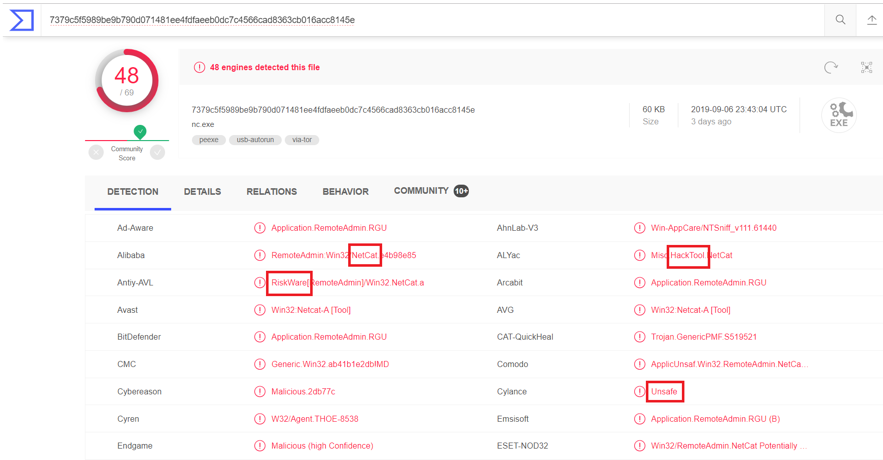
\includegraphics[width=0.99\textwidth]{./figures/Image1.png}
  \caption{\label{fig:1} An illustration of a VirusTotal analysis of Netcat.}
\end{figure}

Malware context is absolutely fundamental during analysis\cite{ContextBasedMalware}\cite{LearningFromContext} so, it must to be
included in the collected samples. The concept of malware sample is broad,
since its nature consists of a composition of miscellaneous elements\cite{ResidentViruses}\cite{FilelessAttacks}\cite{AdvacedVolatileThreat}. We must,
therefore, include different kind of elements (memory dumps, files, pictures
and circuit specifications in case of hardware malware, network traffic
captures, environment variables, etc.) and to enrich these elements with
metadata to indicate the analyst what exactly is any kind of element
appended as metadata as necessary.

In contradiction with any definition of ``malware'', currently a ``malware
sample'' is any kind of file that, potentially, could be malware. In other
words, and to keep it simple, malware samples are not always malware. Let us
clarify this issue next.

\section{The state of the art in malware samples}
\label{sec:soa}

It is known that intelligence tools simply store files, without any rigor of
selection beyond self-tagging by the user who, while it is true, accepts the
EULA (End User License Agreement), probably desiring strongly that potential
sensitive data are properly encrypted.

In the same way, antimalware solutions also take malware samples from the
system of its clients and, with high probability, all the undetected and
unknown elements, because new detections cannot come from other place than the
knowledge acquired from the unknown and undetected samples. Therefore, those
files are paradoxically also called malware samples. This is not a new
thing. For instance, Kaspersky Antivirus has starred the news not long ago on
this issue\cite{RussianStoleNsaSpySecrets}\cite{KasperskyToolForSpying}.  This
highlights that pointing to Kaspersky Antivirus as espionage tool by EE.UU and
EU is not other thing than to accidentally discover the general lack of
current malware sample treatment in general, not by a specific company or
product. In other words, a treatment which does not take into account, among
other issues not at all negligible, data confidentiality and user privacy.

This incident meant great losses, leading Kaspersky to create a ``Transparency
Center''\cite{KasperskyTransparencyCenter} and Eugene Kaspersky, CEO of Kaspersky Lab, to publish many releases like
this: ``We’re even willing to meet with any of them and give them our source
code to thoroughly review it, as we’ve got nothing to
hide''\cite{EugeneKasperskyBlog2017}. Certainly, Kaspersky antivirus is not a spy tool by itself (as happens with
any software piece, it depends on the context, it depends on who uses it), you
can check the entire source code line by line and you will not notice
specifically designed code for espionage, but you will notice the real issue:
samples treatment! And no direct actions were taken in this sense by antivirus
industry because, if it is not well done, it can reduce the protection rate
that, unfortunately, is the only thing the customer demands.

We reproduce as en example two EULA blocks chosen at random because to quote
all will be too much extensive and repetitive. These are quite similar for all
antivirus companies and products.

\begin{tcolorbox}
  \small
  12.1 The Software or Support may employ applications and tools to collect
  Personal Data, sensitive data or other information about Company and End
  Users (including End Users’ name, address, e-mail address and payment
  details), their computers, files stored on their computers, or their
  computers’ interactions with other computers (including information
  regarding network, licenses used, hardware type, model, hard disk size, CPU
  type, disk type, RAM size, 32 or 64 bit architecture, operating system
  types, versions, locale, BIOS version, BIOS model, total scanners deployed,
  database size, system telemetry, device ID, IP address, location, content,
  McAfee products installed, McAfee components, processes and services
  information, frequency and details of update of McAfee components,
  information about third party products installed, extracts of logs created
  by McAfee, usage patterns of McAfee products and specific features, etc.)
  (collectively,
  Data).\footnote{\href{https://www.mcafee.com/enterprise/en-us/assets/legal/end-user-license-agreements-en-us.pdf}{\texttt{https://www.mcafee.com/enterprise/en-us/assets/legal/end-user-license-agreements-en-us.pdf}}}
  
  \tcblower
  SECTION B. CONDITIONS REGARDING DATA PROCESSING

  Provision of information (if applicable) In order to enhance the protection
  of information and improve the quality of the Software and services, You
  agree to automatically provide Kaspersky Lab with the following information
  of a statistical and administrative nature: information about installed
  programs, license data, information on detected threats and infections,
  checksums of processed objects, technical information about the Computer and
  devices connected to it, information about online activity of the device as
  well as You agree that such information can be provided to third-party
  service providers. More information is available at help.kaspersky.com.  In
  order to identify new information security threats and their sources,
  enhance the operational protection of Users of the Software, and improve the
  quality of the product, You agree to automatically provide Kaspersky Lab
  with information specified in the Terms of Use of Kaspersky Security
  Network.  Also, You can activate and deactivate the Kaspersky Security
  Network service at any time in the Software settings window.  You further
  acknowledge and agree that any information gathered by Rightholder can be
  used to track and publish reports on security risk trends at the
  Rightholder’s sole and exclusive discretion.  If you do not wish to provide
  information to the Kaspersky Security Network service, You should not
  activate the Kaspersky Security Network service. If service is already
  activated, you should immediately de-activate the Kaspersky Security Network
  service.

  Kaspersky Lab protects the information received in accordance with
  applicable governing law and Kaspersky Lab's rules. Data is transmitted over
  a secure channel.\footnote{\href{https://products.s.kaspersky-labs.com/homeuser/kav2020/20.0.14.1085abc/english-INT-0.2007.0/3231373433327c44454c7c4e554c4c/eula_en.txt}{\texttt{https://products.s.kaspersky-labs.com/homeuser/kav2020/20.0.14.1085abc/english-INT-0.2007.0/3231373433327c44454c7c4e554c4c/eula_en.txt}}}
\end{tcolorbox}
As you can read from its own words: sensitive data is collected. You can check
not only literature but also the code to verify this.

\section{Antivirus telemetry}

\subsection{Analysis}
Our starting hypothesis is that any antimalware solution is an espionage tool
in potential, and that not only files are sent to the server but also
intelligence information that can be used to spy the users.

Let us do some reverse engineering on an antivirus product in order to know
what kind of information is sent to the company. Let us do this with
\texttt{Malwarebytes} because telemetry DLL is very easy to identify, this is
actually the main reason to chose this antivirus product for investigating the
issue.

\begin{figure}[t]
  \centering
  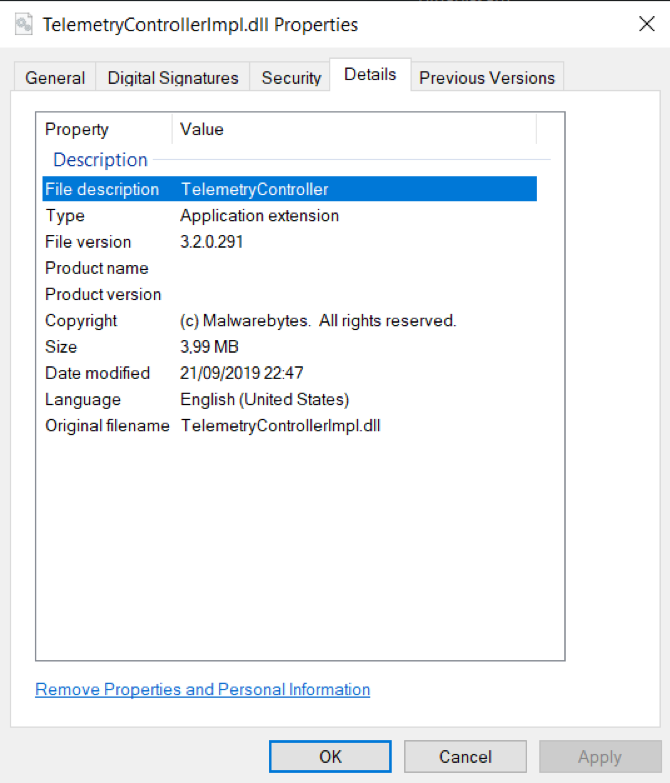
\includegraphics[width=0.85\textwidth]{./figures/ControllerImpl}
  \caption{\label{fig:ControllerImpl} Reverse engineering in
    \texttt{Malwarbytes}.}
\end{figure}
The file responsible of \texttt{Malwarebytes} antivirus telemetry is the
\begin{tcolorbox}
  \texttt{TelemetryControllerImpl.dll}
\end{tcolorbox}
shown in Figure~\ref{fig:ControllerImpl}. If we take a look at the exported
functions, we can see what kind of information is collected
(Figure~\ref{fig:ExportedFunction}).

\begin{figure}
  \centering
  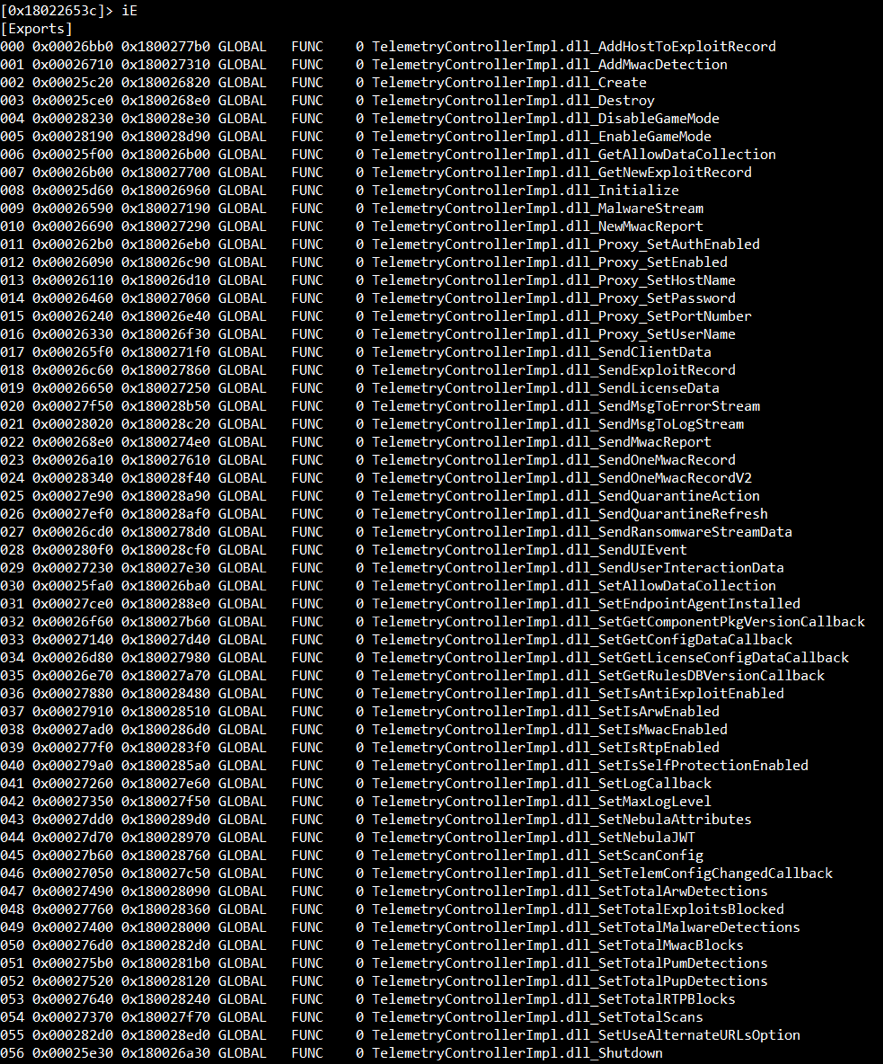
\includegraphics[width=0.85\textwidth]{./figures/ExportedFunction}
  \caption{\label{fig:ExportedFunction} Exported functions.}
\end{figure}

This list of exported function names seems to be self-explanatory, and it
reveals without obfuscation what kind of information is sent. It can be
summarized as follows.
\begin{itemize}
\item Malware information (ransomware is treated in its own specific way).
\item Exploits information.
\item Client data.
\item License data.
\item Error information.
\item Quarantine information.
\item Statistics.
\end{itemize}
We can also contrast the summary developed above with every of the third endpoint path
names of the \texttt{Malwarebytes} telemetry exposed API, shown in Figure~\ref{fig:api}.
\begin{figure}[t]
  \centering
  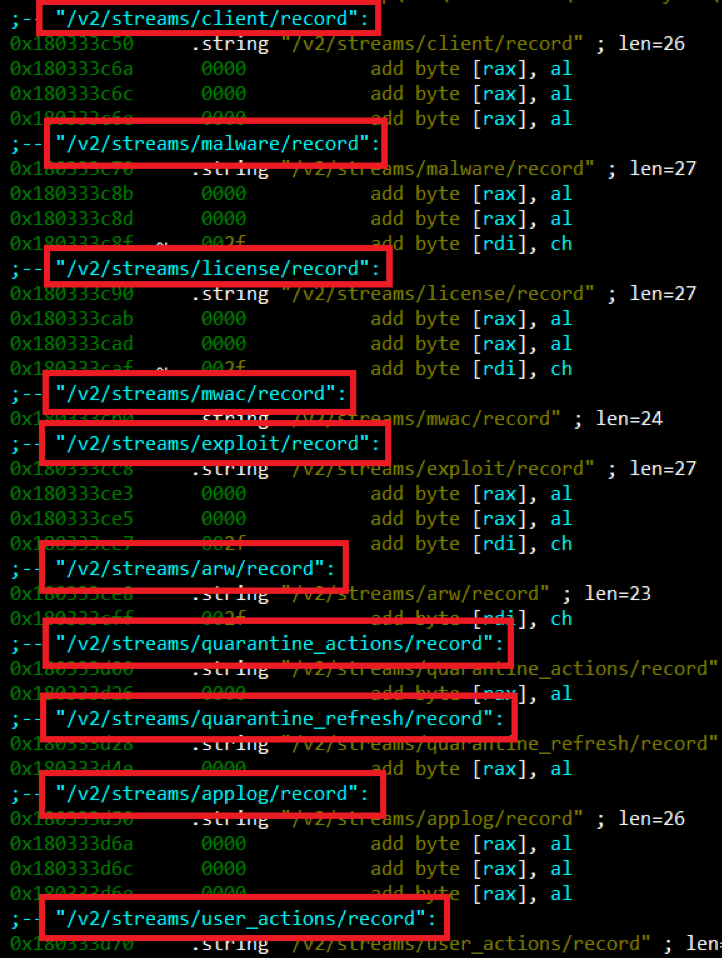
\includegraphics[width=0.80\textwidth]{./figures/Malwarebytes}
  \caption{\label{fig:api} \texttt{Malwarebytes} telemetry API.}
\end{figure}
The endpoint path is the following:
\href{https://telemetry.malwarebytes.com/api}{\texttt{https://telemetry.malwarebytes.com/api}}
and, as an off-topic observation, the development endpoint is also publicly
exposed:
\href{https://telemetry.dev.malwarebytes.com/api}{\texttt{https://telemetry.dev.malwarebytes.com/api}}. 

We can also examine some function of those (\texttt{SendMwacReport}, for
instance, has an interesting name) in order to understand how are samples
treated in terms of confidentiality. This function sends a JSON file
\texttt{mwcstream.json} using Microsoft Winsocks library.
\begin{figure}[h]
  \centering
  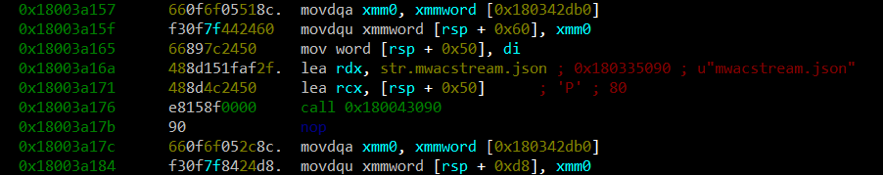
\includegraphics[width=0.99\textwidth]{./figures/mwcstream}
\end{figure}

The function responsible of the ``send'' action is
\begin{tcolorbox}
\texttt{TelemetryControllerImpl::SendMwacReport}
\end{tcolorbox}
as shown in the following disassembly listing:
 \begin{figure}[h]
  \centering
  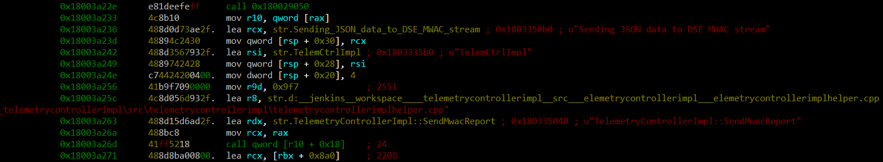
\includegraphics[width=0.99\textwidth]{./figures/SendMwacReport}
\end{figure}

We can take another function from the list and we can see that all information
is sent in the same way. It uses also a JSON file (in this case it is named
\texttt{malwarestream.json}):
\begin{figure}[h]
  \centering
  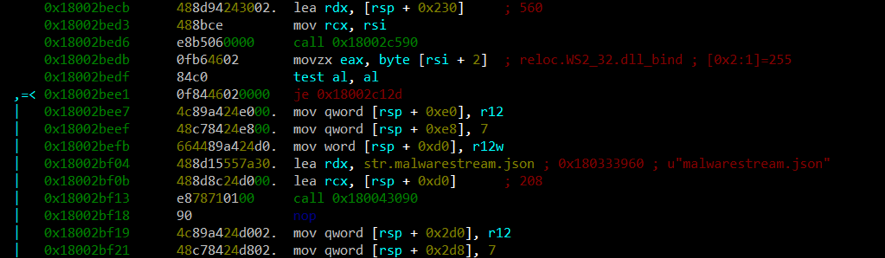
\includegraphics[width=0.99\textwidth]{./figures/malwarestream}
\end{figure}

And finally the appropriate report sending function for this kind of JSON
structure, \texttt{TelementryControllerImpl::ReportMalwareStream} in this
case:
 \begin{figure}[h]
  \centering
  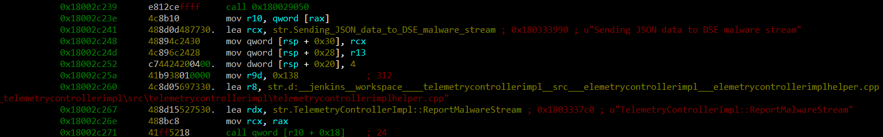
\includegraphics[width=0.99\textwidth]{./figures/ReportMalwareStream}
\end{figure}

Our next step is debug \texttt{Malwarebytes} in order to see how this JSON
looks like. For instance, we can break in some point inside the function
\texttt{SendOneMwacRecordV2} after analyzing (on demand) a file infector, and
see the information.
\begin{figure}[h]
  \centering
  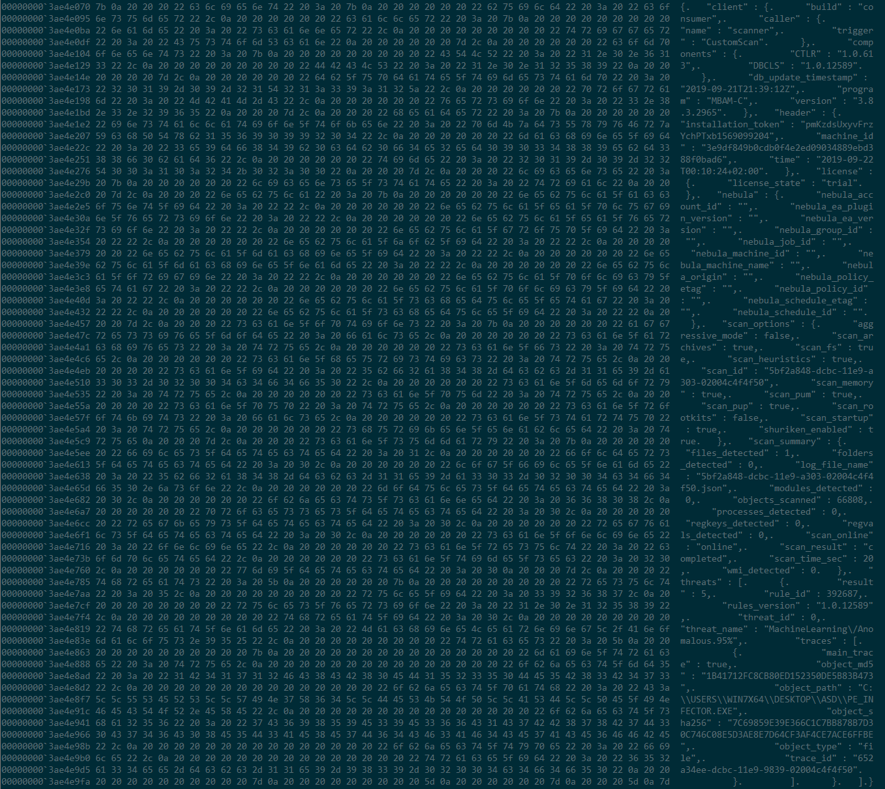
\includegraphics[width=0.99\textwidth]{./figures/Debug1}
\end{figure}
As you can see, apart of malware sample itself, other information is collected
separately, unencrypted and stored in a non-standard format. We remark that
the computer where these tests have been performed can be easily tracked by
checking the unique identifier \texttt{machine\_id}. Into the binary
\texttt{.rdata} section a series of WMI queries do exist for machine
identification purposes.
\begin{figure}
  \centering
  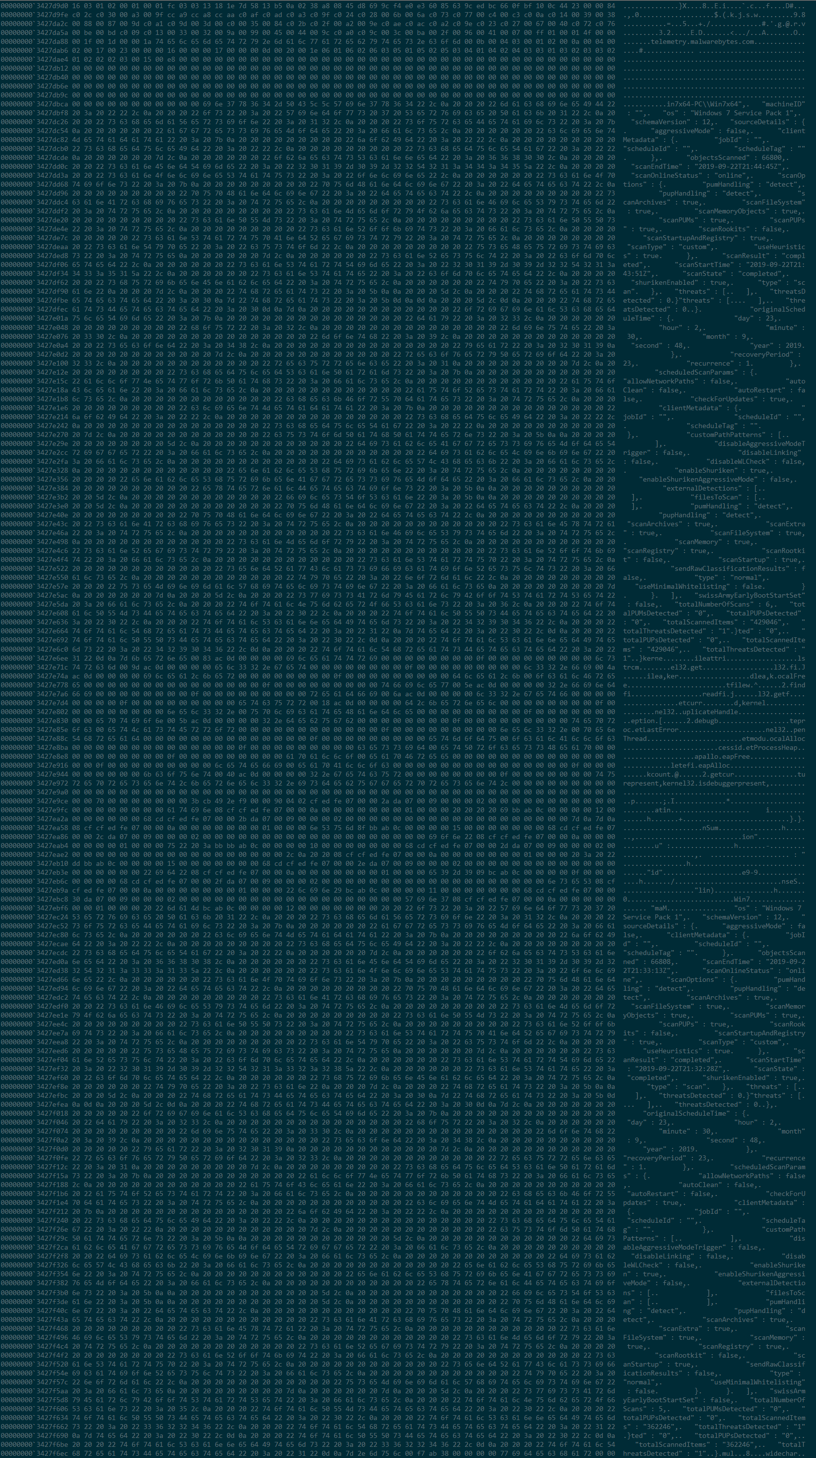
\includegraphics[width=0.85\textwidth]{./figures/Debug2}
  \caption{\label{fig:malwarebytes-debug} Debugging \texttt{Malwarebytes}.}
\end{figure}

\begin{tcolorbox}
  \small
\begin{verbatim}
SELECT Index, MACAddress, Name FROM Win32_NetworkAdapter 
       where AdapterTypeId=0
SELECT UUID FROM Win32_ComputerSystemProduct
SELECT processorID FROM win32_processor
SELECT SerialNumber FROM Win32_BIOS
SELECT Signature FROM Win32_DiskDrive WHERE Index=%u
SELECT serialNumber FROM Win32_PhysicalMemory
SELECT SerialNumber FROM Win32_DiskDrive WHERE Index=%u
\end{verbatim}
\end{tcolorbox}

Since Microsoft Winsock functions are used for network communications, we can
also break in \texttt{Send} and \texttt{SendTo} functions and show de buffer
content before telemetry data are sent
(Figure~\ref{fig:malwarebytes-debug}). It is as easy as stated because the
\texttt{Malwarebytes} self-defense is not enabled just after installing the
product, a really hilarious security bug which can be used to attack the
debugger without bypassing any kind of protection.


The file responsible of Malwarebytes antivirus cloud functionality is the
\texttt{CloudControllerImpl.dll}.
\begin{figure}[h]
  \centering
  \includegraphics[width=0.7\textwidth]{./figures/CloudcontrollerImpl}
\end{figure}


Let us follow the same analysis steps with this file. Now, export listing looks as
follows:
\begin{figure}[h]
  \centering
  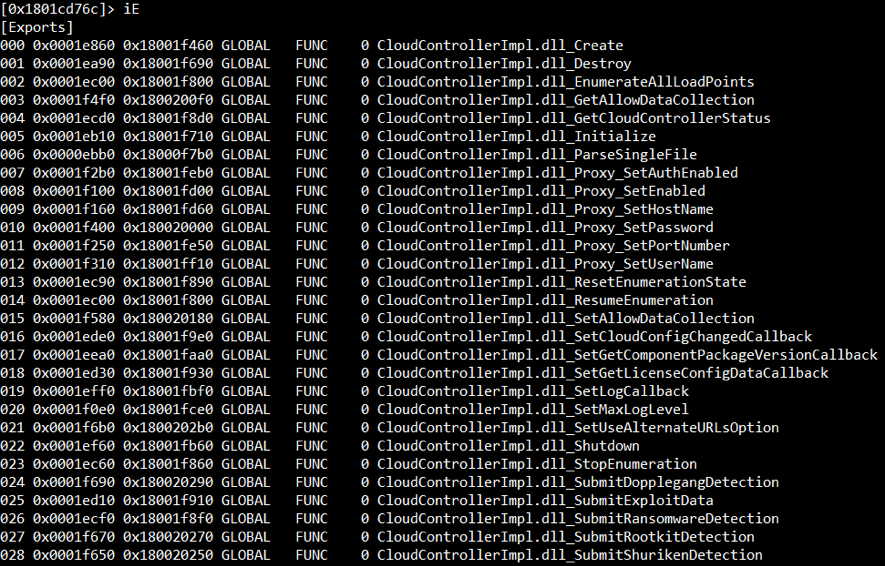
\includegraphics[width=0.7\textwidth]{./figures/ExportListing}
\end{figure}

There are five functions at the very end of the screenshot named starting by
the prefix \texttt{Submit}. Those functions are responsible of submitting
files and memory chunks to the \texttt{Malwarebytes} cloud storage, but those
functions are only called when upgrading to the premium version of the
product\cite{MalwarebytesUserGuide}.  
\begin{figure}[h]
  \centering
  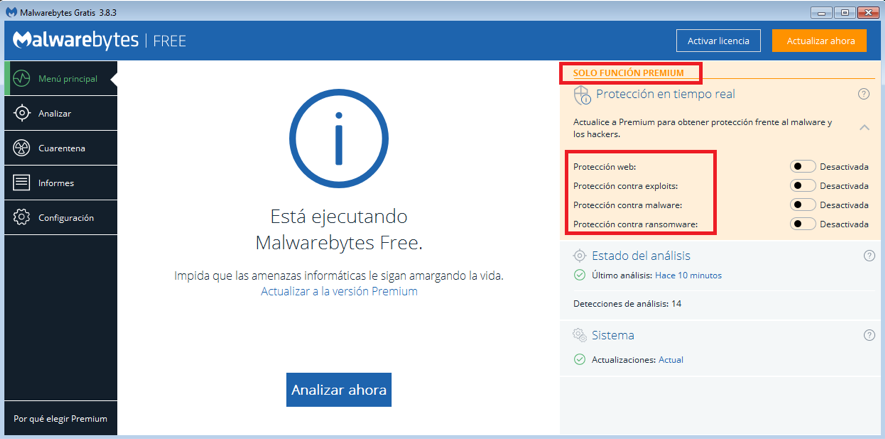
\includegraphics[width=0.99\textwidth]{./figures/MalwareBytesFree}
\end{figure}

The reader should know what ``exploit'', ``ransomware'', and ``rootkit'' mean,
but there are two function names which maybe seem a little stranger:

\noindent\texttt{SubmitDopplegangDetection} and \texttt{SubmitShurikenDetection}
because they are \texttt{Malwarebytes} specific terms. The first one,
\texttt{SubmitDopplegangDetection}, as you can see in the following picture,
is used to send ``scam'' detections:
\begin{figure}[h]
  \centering
  \includegraphics[width=0.75\textwidth]{./figures/Scamdetection}
\end{figure}

But \texttt{SubmitShurikenDetection} is much more interesting for us, because
it is used to send heuristically detected samples, meaning, by definition,
that false positives will absolutely happens (goodware files are potentially
sent to the cloud storage).
\begin{figure}[h]
  \centering
  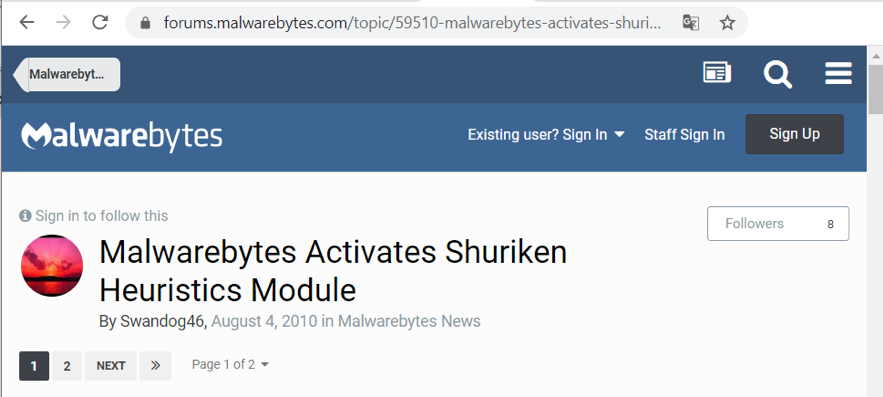
\includegraphics[width=0.75\textwidth]{./figures/SubmitShurikenDetection}
\end{figure}

All of this information is submited to the following endpoints:
\begin{tcolorbox}
  \small
  \href{https://bactem-staging.mwbsys.com/files}{\texttt{https://bactem-staging.mwbsys.com/files}} \\
  \href{https://staging-blitz.mb-cosmos.com/}{\texttt{https://bactem-staging.mwbsys.com/files}} \\
  \href{https://blitz.mb-cosmos.com/}{\texttt{https://blitz.mb-cosmos.com/}} \\
  \href{https://static-blitz.mb-cosmos.com/}{\texttt{https://static-blitz.mb-cosmos.com/}}
  \\ 
  \href{https://blitz.mb-cosmos.com/}{\texttt{https://blitz.mb-cosmos.com/}} \\
  \href{https://static-blitz.mb-cosmos.com/}{\texttt{https://static-blitz.mb-cosmos.com/}}
\end{tcolorbox}
If the reader is interested about where those files are stored, we can also
answer this question. These files are stored in the server referenced by the
following IP address: \texttt{3.229.68.76} and it corresponds to Amazon Data
Services NoVa:
%\begin{figure}[h]
%  \centering
%  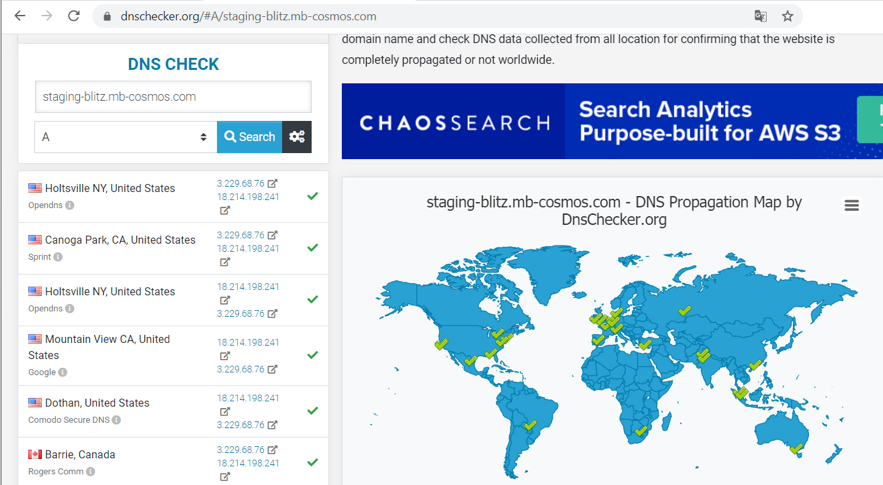
\includegraphics[width=0.75\textwidth]{./figures/DNScheck}
%\end{figure}

\begin{figure}[h]
  \centering
  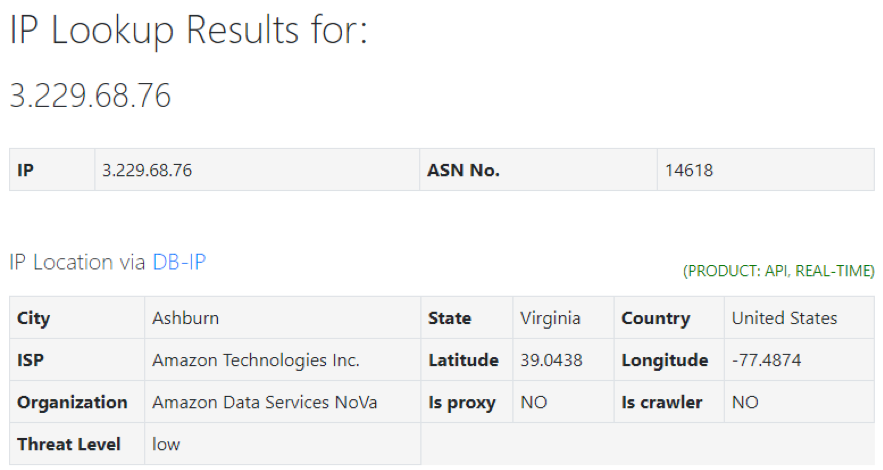
\includegraphics[width=0.75\textwidth]{./figures/Lookup}
\end{figure}

This is an important point because the code is developed using Amazon S3
API\cite{AmazonS3RestApi}.
The following is a little fragment of the \texttt{Shuriken} sending function:
\begin{figure}[h]
  \centering
  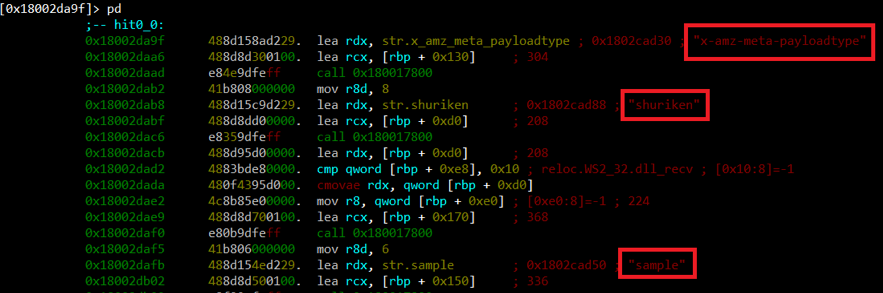
\includegraphics[width=0.99\textwidth]{./figures/Shuriken}
\end{figure}

As you can see, \texttt{x-amz-meta-payloadtype} is the ``payloadtype'' custom
metadata parameter prefixed as specified by Amazon S3 API, and the rest means
that a \texttt{Shuriken} sample submission is happening.
\begin{figure}[h]
  \centering
  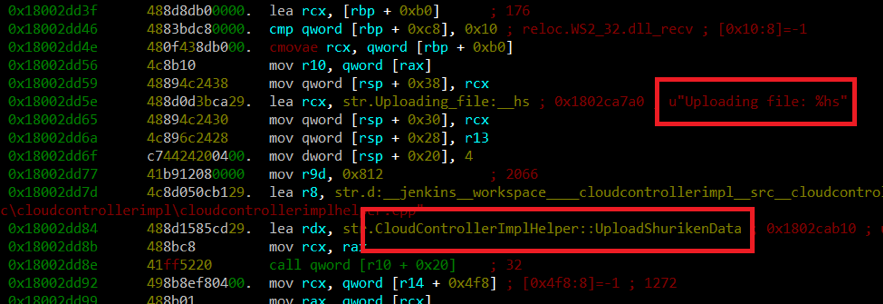
\includegraphics[width=0.99\textwidth]{./figures/Shuriken2}
\end{figure}

Thus, we have identified the mechanism used to send samples and telemetry data
to the \texttt{Malwarebytes} cloud server. Another interesting thing is to
know how file and memory samples are chosen by this product in order to keep
them in the server. Following the natural analysis flow, some interesting
functions are located into \texttt{MBAMService.exe} which finally relies on
\texttt{CloudControllerImpl.dll} where all the hard job takes place.
\begin{figure}[h]
  \centering
  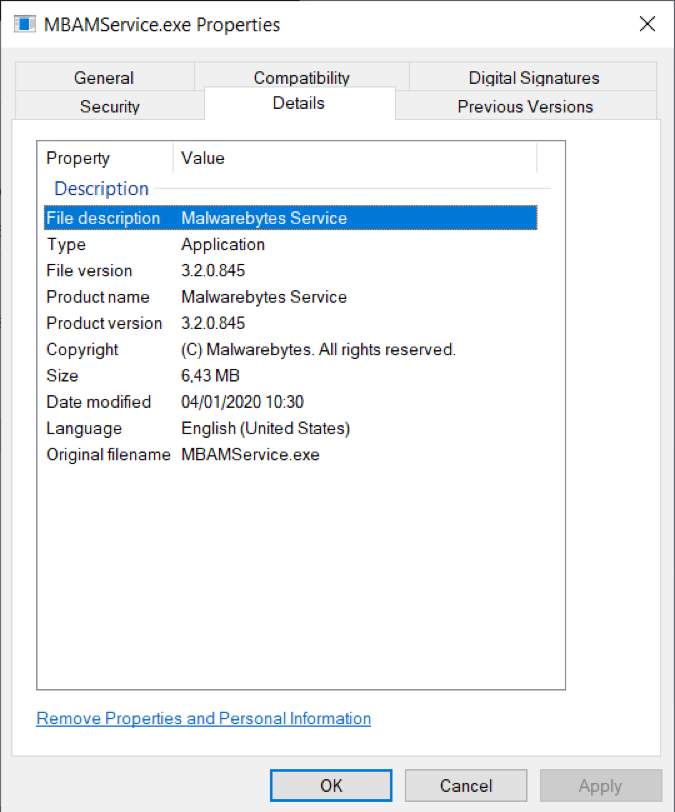
\includegraphics[width=0.75\textwidth]{./figures/MBAMService}
\end{figure}

There are a lot of callbacks into this binary image. Two of them make
reference to cloud submission and telemetry submission, specifically:
\begin{figure}[h]
  \centering
  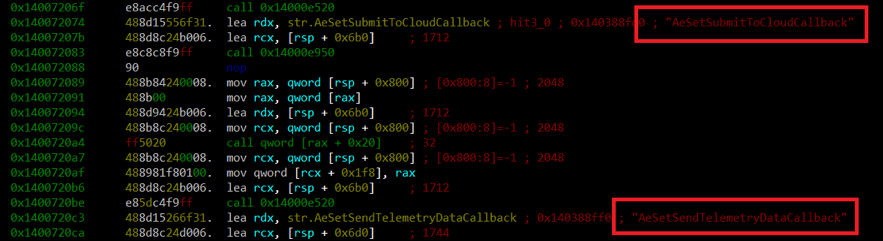
\includegraphics[width=0.99\textwidth]{./figures/Callbacks}
\end{figure}

If reader is really interested about how \texttt{Malwarebytes} heuristically
chooses files to be sent to the cloud storage, remember that when using
heuristics, by definition, no categorical conclusions are possible so false
positives will happen. Therefore, confidential files in addition to potential
malware embedding confidential data could be sent to the server. It is
recommended to the restless reader to disassemble
\texttt{CloudControllerImpl.dll} by his/her own to perform a further analysis.

At this point, it is necessary to install \texttt{Malwarebytes} Premium in
order to investigate the file submission features. We obtained a trial\cite{MalwarebytesPremium} license
for a limited period.  In this Premium Trial version, real-time features are
available. We noticed that this \texttt{Malwarebytes} version has more sample
submission routines, and identified the following sample submission exports in
the \texttt{CloudControllerImpl.dll} library file:
\begin{enumerate}
\item \texttt{SubmitDDSSample}
\item \texttt{SubmitDopplegangDetection}
\item \texttt{SubmitExploitData}
\item \texttt{SubmitMWACDetection}
\item \texttt{SubmitQuarantineRestoreItem}
\item \texttt{SubmitRansomwareDetection}
\item \texttt{SubmitRootkitDetection}
\item \texttt{SubmitShurikenDetection}
\end{enumerate}
The first thing we are interested in to investigate is how samples are
submitted. To this end, we executed a portable executable file infector and
broke into the \texttt{send} function of \texttt{WS2\_32.dll} to see how the
buffer content looks like.
\begin{figure}[h]
  \centering
  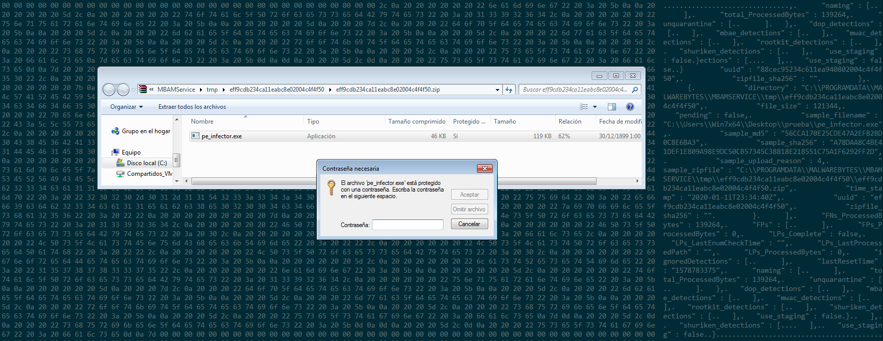
\includegraphics[width=0.99\textwidth]{./figures/Submission}
\end{figure}

As you can see in the JSON structure of the previous image, the sample file is stored into the following location:

\noindent{\small\verb|{C:\PROGRAMDATA\MALWAREBYTES\MBAMSERVICE\tmp\{hash_sha256}\{hash_sha256}.zip|}

\noindent This is a PKZIP file encrypted with the typical malware sample
password: ``infected''\cite{ZeltserShareMalware}.  And it will be sent to the Amazon server
\begin{tcolorbox}
  \texttt{btoc-samples-prod.s3.amazonaws.com}.
\end{tcolorbox}
The hypothesis that files are submitted is confirmed. The other thing we are
interested in to investigate is if \texttt{Malwarebytes} indiscriminately
submits all files or not.  Since a ``hello world'' program should never lead
to a false positive, if it is submitted, it can be assumed that submissions
are done indiscriminately.
\begin{figure}[h]
  \centering
  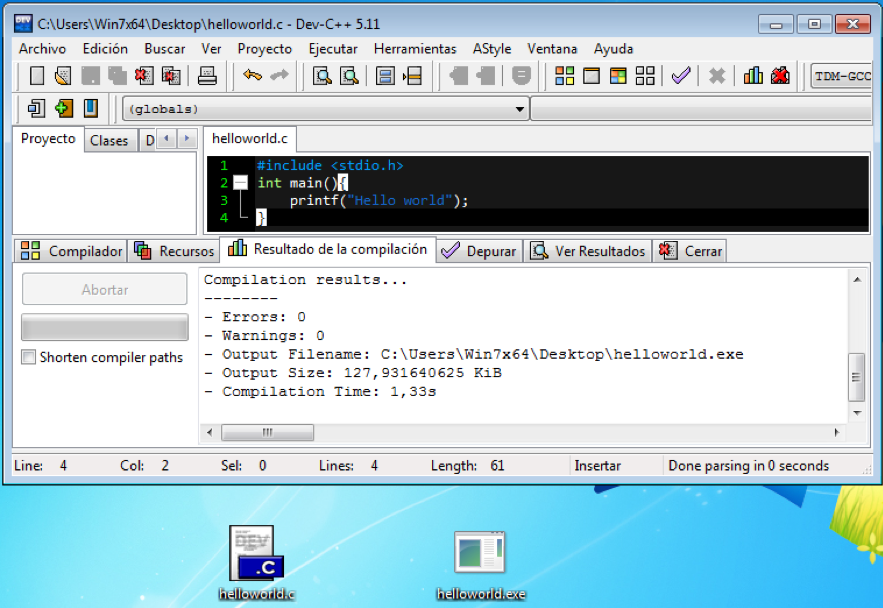
\includegraphics[width=0.99\textwidth]{./figures/HelloWorld}
\end{figure}

The experiment result indicated that, when \texttt{helloworld.exe} was
executed, some information was sent to \texttt{Malwarebytes} by using
\texttt{WS2\_32.dll} library \texttt{send} function with the call flow coming
from somewhere inside \texttt{RTPControllerImpl.dll}. This library contains
the following strings: \pagebreak
\begin{figure}[h]
  \centering
  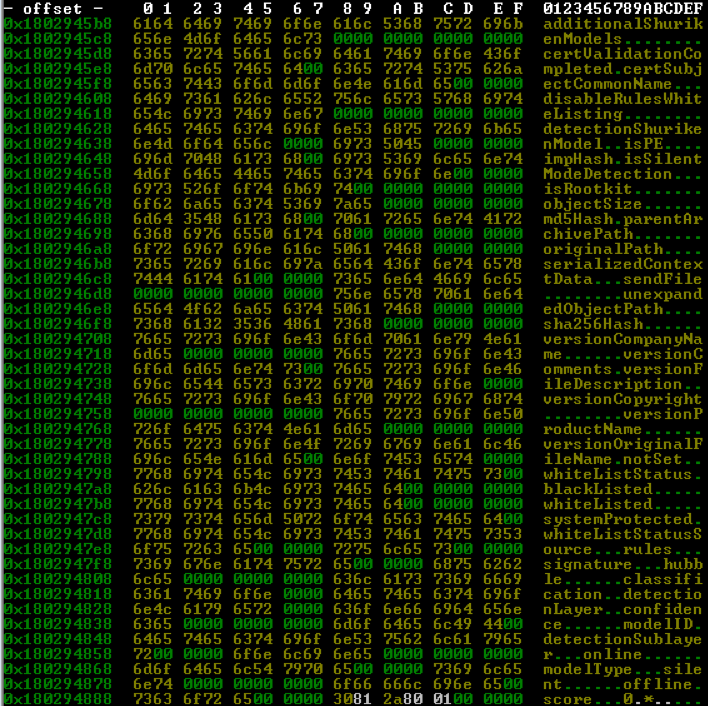
\includegraphics[width=0.85\textwidth]{./figures/Strings}
\end{figure}

\begin{figure}
  \centering
  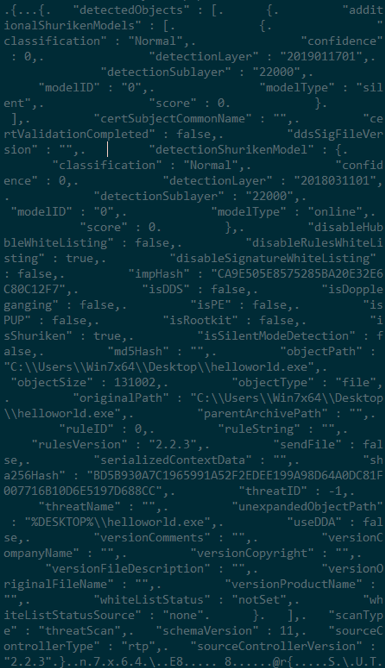
\includegraphics[width=0.6\textwidth]{./figures/ExperimentJSON}
  \caption{\label{fig:ExperimentJSON} Sample of the JSON experiment.}
\end{figure}
A function of \texttt{RTPControllerImpl} uses it to generate the
JSON. Experiment JSON looks as in Figure~\ref{fig:ExperimentJSON}.  So,
\texttt{Malwarebytes} Premium sends file samples only if it suspects a file
could be infected (a \texttt{sample\_upload\_reason} field do exist into the
JSON structure).  If the file is not a suspicious one, \texttt{Malwarebytes}
Premium sends information about the file (like the file path and something
like this) but not the file content itself. Anyway, subjectively, in our
opinion, executable files leak a lot of information about the user behavior.

\subsection{Conclusions}
The reverse engineering of the \texttt{Malwarebytes} antivirus products
reveals that these are not especially intrusive. They are classical
antiviruses with cloud features which send suspicious files and telemetry to
the cloud server just for purposes of comparison.

Our analysis indicates that some files (but, with congratulations to
\texttt{Malwarebytes}, not an indiscriminate massive volume of goodware ones)
are sent to the company's cloud server powered by Amazon.

Sample submission is done by using a PKZIP file protected with the typical
malware sample password: ``infected''\cite{ZeltserShareMalware}. And metadata information (telemetry) is
sent separately using a JSON format.  On the other hand, the most important
thing is that accessed goodware information is sent, the user is unambiguously
identified and some information is collected apart of the sample file itself.
If such collected information were accessed, for instance, by a third party
like an unethical employee or a government intelligence agency (which maybe
collaborates with the antivirus company and could take advantage of this fact)
they could track a specific user (or users, in general) and combine this
information with other databases (including another antivirus products)\cite{KasperskyBoundariesOfTrust}.
\texttt{Malwarebytes} could substantially improve its system by removing both,
the compressed samples system and the telemetry data. Instead, it could
progressively add sample and telemetry support to the UMSE dynamic linking
library and call to it before submitting samples.

\section{Cyber threat hunting telemetry and samples submission}

\subsection{Analysis}

Cyber threat hunting is defined as follows: ``the process of proactively and
iteratively searching through networks to detect and isolate advanced threats
that evade existing security solutions''.

In practice, cyber threat hunting means to capture as many events as possible,
correlate them and send reports of them all the time. All the magic can be
summarized in one sentence: everything can be detected if everything is
real-time reviewed.
\begin{figure}
  \centering
  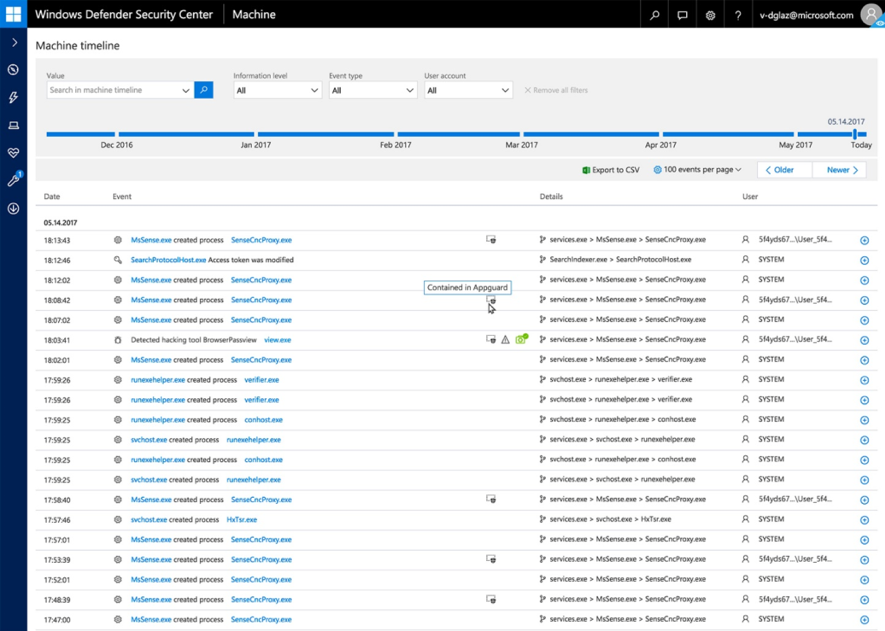
\includegraphics[width=0.75\textwidth]{./figures/WindowsDefender}
  \caption{\label{fig:WindowsDefender} A screenshot of WindowsDefender.}
\end{figure}

For instance, Windows Defender Advanced Threat Protection captures the
following information\cite{MicrosoftDefenderAtp2020}, as shown in Figure~\ref{fig:WindowsDefender}:\footnote{\href{https://docs.microsoft.com/en-us/windows/security/threat-protection/microsoft-defender-atp/advanced-hunting-schema-reference}{https://docs.microsoft.com/en-us/windows/security/threat-protection/microsoft-defender-atp/advanced-hunting-schema-reference}}
\begin{enumerate}
\item Alerts on Microsoft Defender Security Center.
\item Machine information, including OS information.
\item Network properties of machines, including adapters, IP and MAC
  addresses, as well as connected networks and domains.
\item Process creation and related events.
\item Network connection and related
  events.
\item File creation, modification, and other file system events.
\item Creation and modification of registry entries.
\item Sign-ins and other authentication events.
\item DLL loading events.
\item Multiple event types, including events triggered by security controls
  such as Windows Defender Antivirus and exploit protection.
\end{enumerate}
The idea is the same for all products. Event correlation is an important
feature. Check Figure~\ref{fig:CarbonBlack}, as an example, taken out of from the
\texttt{Carbon Black}\cite{CarbonBlack2017} tool.
\begin{figure}
  \centering
  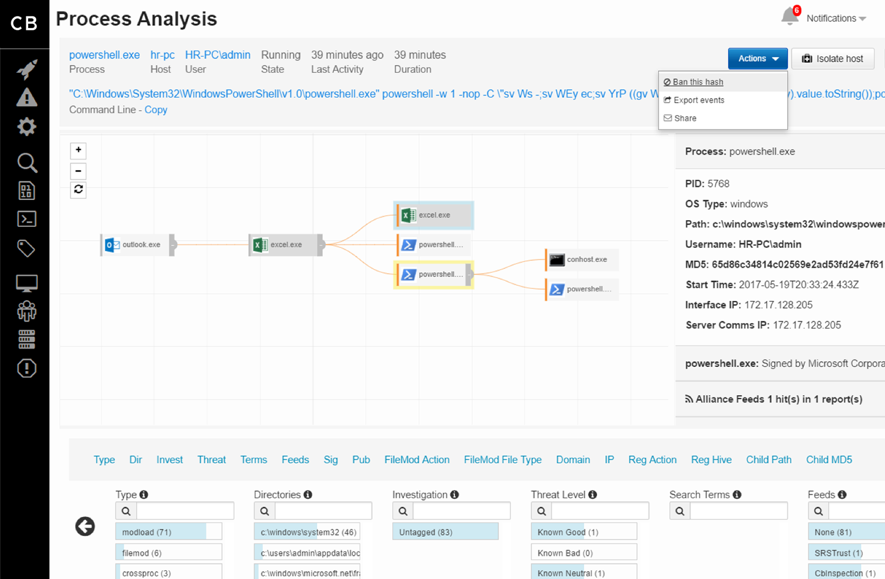
\includegraphics[width=0.99\textwidth]{./figures/CarbonBlack}
  \caption{\label{fig:CarbonBlack} Source: \href{https://www.carbonblack.com/wp-content/uploads/2017/04/BanHash-B.png}{\texttt{https://www.carbonblack.com/wp-content/uploads/2017/04/BanHash-B.png}}}
\end{figure}

\subsection{Conclusion}

It is hard to imagine a more aggressive kind of security tools in terms of
user data confidentiality. More detections but unjustifiably much less
confidentiality.  You can check pictures publicly available in Google of this
kind of tools, most of them will be carefully chosen by the manufacturer
(meaning that the aggressive behavior will be as hidden as possible) but if
one watches the dashboard containing event logs of those tools, one will soon
realize how powerful they are in terms of surveillance. You will see a steady
stream of events unrelated to malware.  Threat hunting tools could also
substantially improve their system by adding events, files, processes,
registry keys and support for system elements into the UMSE dynamic linking
library, and by calling to its API before submitting collected data.

\section{Operating system telemetry and samples submission}

\subsection{Analysis}

Next, we want to explore what happens if there are no additional antivirus
software installed in the computer. Must the user be worried about security
products that maybe come built-in the operating system? And, if these are
disabled, must the user be worried about other security products installed in
the local area network (LAN) because of firewall telemetry and sample
submission capabilities?

The Microsoft Windows telemetry DLL file is located in
\begin{tcolorbox}
  \verb|C:\Windows\System32\generaltel.dll|.
\end{tcolorbox}
\begin{figure}[h]
  \centering
  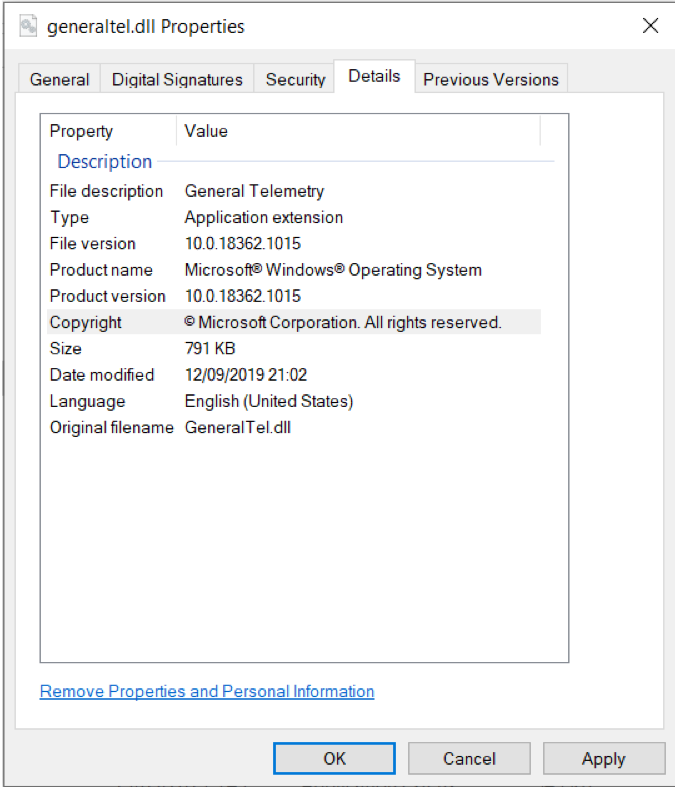
\includegraphics[width=0.6\textwidth]{./figures/WindowsTelemetry}
\end{figure}

And you will readily notice that miscellaneous antivirus, antispyware and
firewall information is sent to Microsoft, where \texttt{Firewall information}
means network information. It is possible to disable all the telemetry but
maybe your LAN neighbor does not do that.
\begin{figure}[h]
  \centering
  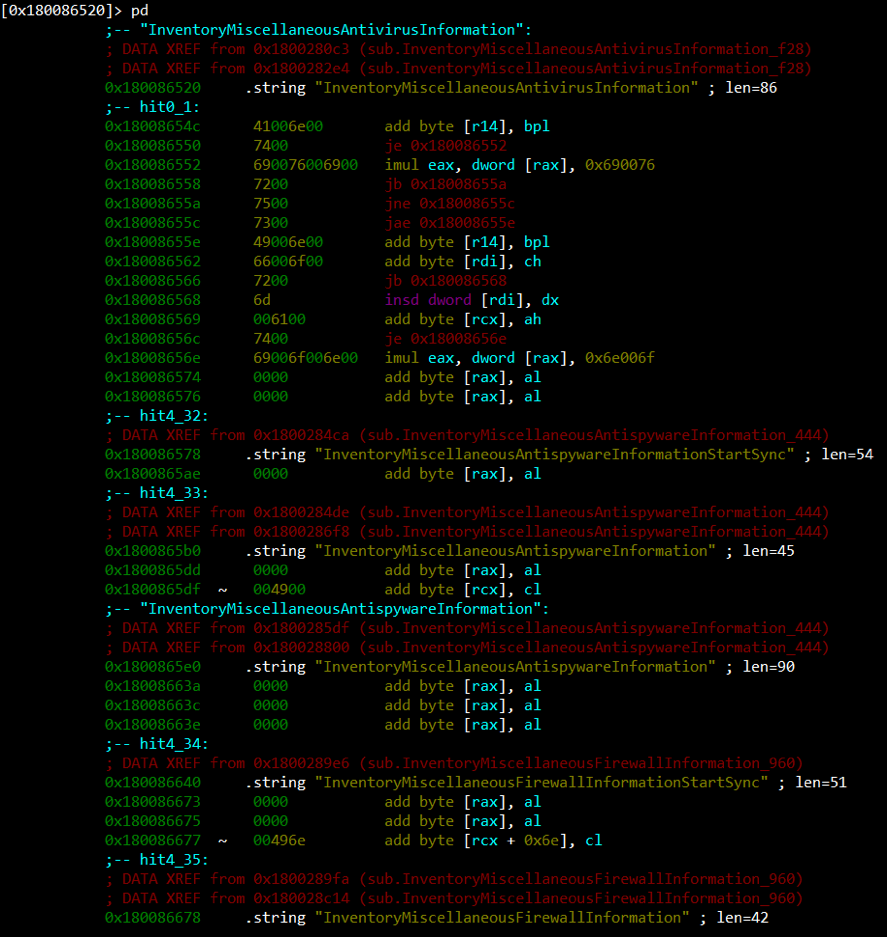
\includegraphics[width=0.99\textwidth]{./figures/MiscellaneousAntivirus}
\end{figure}

The cloud submission features of sample files also do exist and they are
customizable by the user. It is possible to check easily (without reverse
engineering nothing) what kind of information is sent to Microsoft because,
due to open criticism, they released a tool named \texttt{Diagnostic Data
  Viewer}. You can use it immediately for those purposes (Figure~\ref{fig:libUmse}).
\begin{figure}[h]
  \centering
  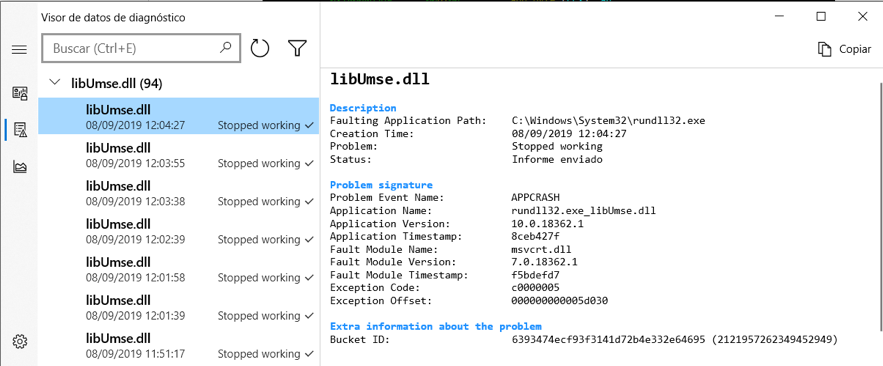
\includegraphics[width=0.75\textwidth]{./figures/libUmse}
  \caption{\label{fig:libUmse} libUmse.dll}
\end{figure}

In the lab computer used for this work, minimum telemetry is allowed which
means that antimalware telemetry is disabled but nevertheless crashes allow
Microsoft to follow the development of this thesis in real-time. Someone might
think that this assessment is unrelated to malware but information about
crashes is also used for this\cite{MicrosoftRdpCrashes2019} (see Figure~\ref{fig:rdp})
purpose.\footnote{\href{https://www.microsoft.com/security/blog/2019/11/07/the-new-cve-2019-0708-rdp-exploit-attacks-explained/}{https://www.microsoft.com/security/blog/2019/11/07/the-new-cve-2019-0708-rdp-exploit-attacks-explained/}}
\begin{figure}[h]
  \centering
  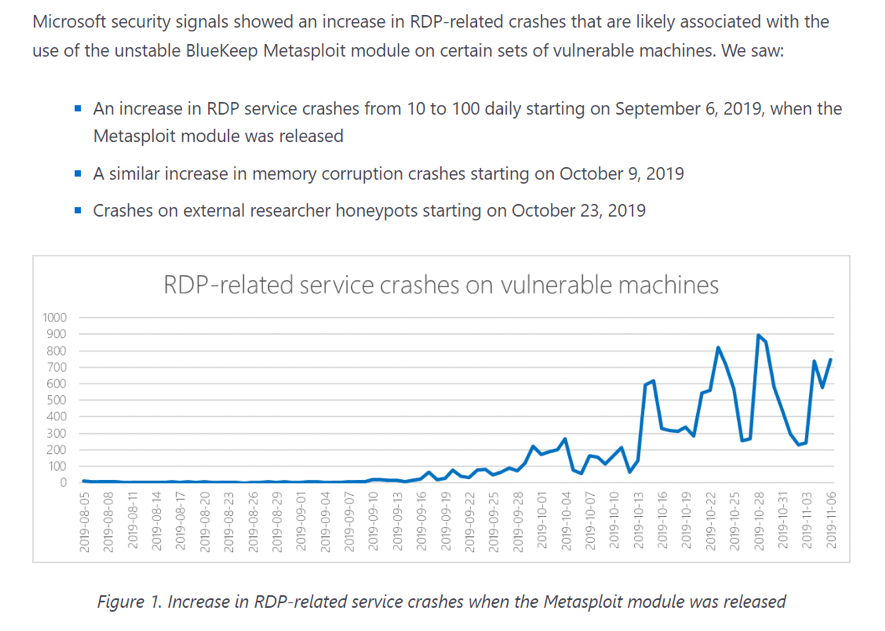
\includegraphics[width=0.8\textwidth]{./figures/RDP}
  \caption{\label{fig:rdp}}
\end{figure}

\subsection{Conclusion}

Some operating systems contain built-in antimalware/firewall/threat hunting
solutions. It is difficult for the common user to disable telemetry
capabilities. A minimum telemetry is required by the operating system (and
seems to be used also for malware purposes). Antivirus, antispyware and
firewall information is sent meaning that also LAN network information can be
revealed.  Operating system antimalware/firewall/threat hunting solutions
could also substantially improve its system by adding events, files,
processes, registry keys and system elements support into the UMSE dynamic
linking library and calling to it before submitting collected data.

\section{Intelligence products}

\subsection{Analysis}

Malware intelligence tools store goodware in, maybe, greater volume than
malware.  \texttt{VirusTotal} is a service which allows you to check if a file
is malware or not by querying a lot of antivirus engines.  If you search,
e.g.,''tutorial pdf'' in Google, (a reasonable random goodware file), the
first result, in this case, is a Python Tutorial PDF. Finally, if you check if
this file does exist in \texttt{VirusTotal}, you can see that it does (really,
a lot of files are in \texttt{VirusTotal}, this can be checked
straightforwardly). So, any person with a \texttt{VirusTotal} paid API account
can download this file, make advanced searches in binaries (including Yara
search) and easily locate files\cite{VirusTotalFileSearch2020}. It is true that people who submits files
accepts the EULA but, as you can see, if you have the paid \texttt{VirusTotal}
API you can download books, software, movies \dots. Those old determined
goodware files, some even signed, will be never removed from storage.

\subsection{Conclusion}

Malware intelligence tools store goodware in, maybe, greater volume than
malware\cite{IntrusionDetectionNetworks}. Those are not malware samples, those are simple, ordinary files.
Intelligence products could also substantially improve its system by adding
encryption support for uncommon and copyrighted likely goodware files (because
those files are not interesting for malware analysis in any way, not even to
be compared with infected files) into the UMSE dynamic linking library. In
this way, only files detected by at least one antimalware engine or a reliable
human should be decrypted and opened to the world.

%%% Local Variables:
%%% mode: latex
%%% TeX-master: "thesis"
%%% End:

\chapter{Universal Malware Sample Encryption (UMSE)}

\section{Current malware sample shortcomings}

It is no surprise, it makes sense. Neither the end user nor the best antivirus
comparators\cite{AVComparatives2020}\cite{AVTest}, not even the most excellent and tested, have ever rated security
tools in this key aspect: confidentiality. The amount of client computer
leaked data by each accomplishes malware detection. When comparing them, they
only take into account some other factors currently much more in dispute. We
will refer to its table columns in the results: ``blocked'', ``user
dependent'', ``compromised'', ``protection rate'' and ``false
alarms''\cite{AVComparativesResults2019}.
  
\begin{figure}[h]
  \centering
  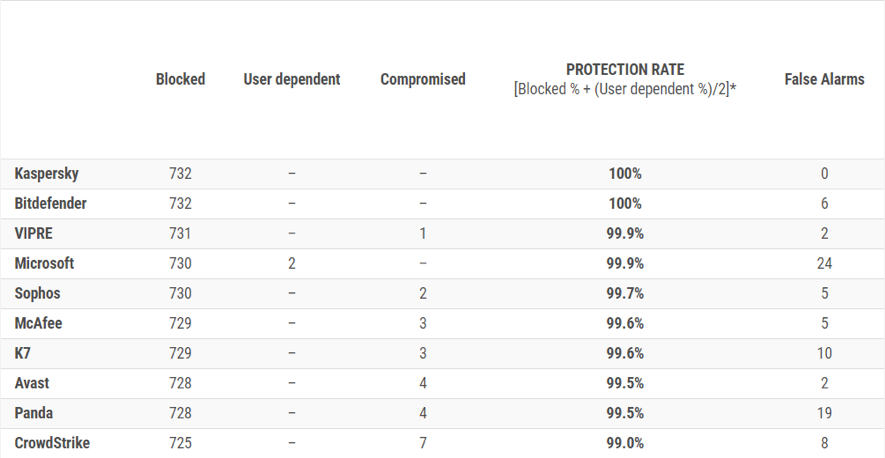
\includegraphics[width=0.99\textwidth]{./figures/MalwareSample}
\end{figure}

Therefore, all antiviruses are good in detection and this explains different
results drawn months apart when comparing them but, how good are they in
confidentiality? Just note how important confidentiality is for the user when
choosing between antimalware products.

Taking up the issue of what malware sample currently is, we should add that,
sometimes, in order to mitigate risks in transport, storage and sample
sharing, this functional file is wrapped in a compression format like PKZIP
and, when supported by such format, maybe encrypted also by the de facto key,
i.e., the symmetric but publicly known key:
``infected''\cite{ZeltserShareMalware}\cite{VXVault2020}\cite{VirusTotalFileSearch2020}\cite{MalShare2020}\cite{VirusShare2020}\cite{VirusBay2020} The following picture shows a
threat intelligence website in which files are downloaded in this way but the
reader should know \texttt{Malwarebytes} uses this mechanisms because it was
analyzed and shown in section~\ref{sec:}
\begin{figure}[h]
  \centering
  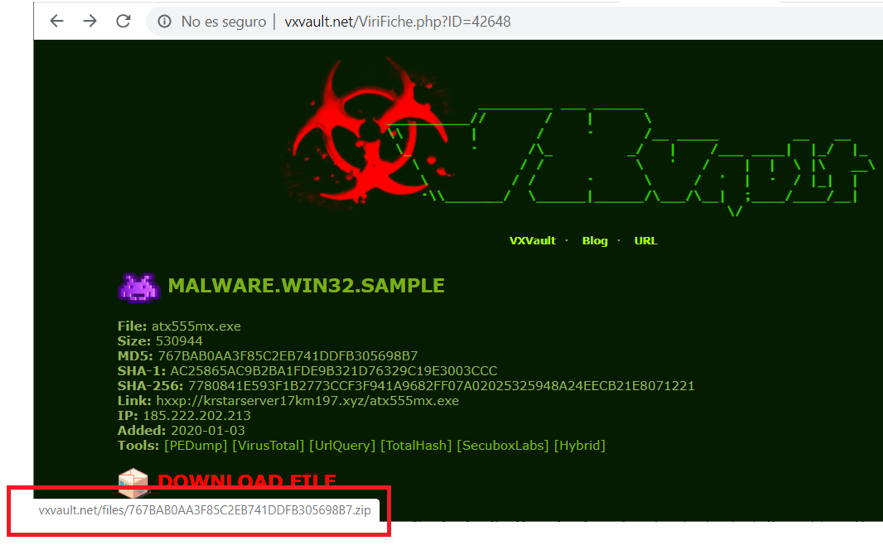
\includegraphics[width=0.99\textwidth]{./figures/ThreatWebsite}
\end{figure}

This way of acquiring and storing malware samples, as is evident, was
improvised but not seriously thought. In summary, the approach has the
following shortcomings:
\begin{enumerate}
\item Identification shortcoming: Given a malware sample, it is not possible
  to know, a priori, if the file is a malware sample or not. It is, at every
  respect, simply a compressed file.

\item Universality shortcoming: A malware sample is not a file. Malware,
  according to UMSE, is an element or a set of elements, hardware, software
  and/or firmware which framed in a context and in a state of its life cycle
  is determinated malicious. Accordingly, a malware element can be
  ``fileless'' or, in a given moment of its life cycle, to be volatile,
  located only in principal memory (like it happens with
  \texttt{DoublePulsar}, to name an example) and this must not be a problem
  when taking a malware sample. To put it differently, the sample must contain
  the element or the set of elements indicating its nature and all of those
  metainformation which is considered necessary.
  
\item Contextualization shortcoming: Context is lost. The sample is usually is
  a file without context. This lost will take unfortunate consequences in
  subsequent phases of the reverse engineering process.

\item Standardization shortcoming: The analyst does not know what kind of
  element is dealing with when he/she gets a sample, or how it came to be a
  sample. A real life example: During compression and decompression processes,
  it usually happens that, for instance, the compression format, being
  arbitrary, does not allow to store all file attributes and enters spurious
  values when decompressed.

\item Confidentiality shortcoming: Potentially confidential data stored in the
  samples is not protected in any way. Therefore, this data will be revealed
  to analysts, companies and intelligence organizations and/or partners or
  whoever malware sample is shared with. This data far exceeds the ``need to
  know'' principle, that is, the amount of information the professional really
  needs in order to do his/her job. We can put an easy-to-understand example
  of this risk. If an office file has aroused malware suspicion and it has
  macros, it is common sense to examine the macros at first and, if the code
  in macros code is not sufficient then, using the concept of encrypted
  malware sample proposed in this work, to decrypt other parts of the file
  content usually more confidential and less malware-prone but keeping a log
  of this decryption operations.
  
\item Authentication shortcoming: It is not possible to determine the
  authenticity of a sample if it was modified after acquisition. Note that
  authentication is also necessary to support encryption in order to guarantee
  confidentiality.
\end{enumerate}

\section{Universal Malware Sample Encryprtion}

\textbf{Universal Malware Sample Encryption format}, (henceforth, UMSE), is a
specific universal file format for malware samples, making efforts in
efficient acquisition, transport and storage which preserves confidentiality,
authenticity and makes possible the potential samples sensitive data access
registration.

\subsection{UMSE universality}

This format is declared to be \textbf{universal} because it supports the
storage of any kind of potential malware sample (contextualized and metadata
enriched) covering any possible state of its life cycle. Expanding, therefore,
the current malware sample concept\cite{ZeltserShareMalware} (limited to files) to a more general
concept which allows the right storage of any element software, hardware
and/or firmware.  Understanding by elements software, hardware and/or
firmware: system processes, program parameters, environment variables,
register entries, network traffic captures, memory content, file paths and
other file system information, integrated circuits photos and schemes, etc.

\subsection{UMSE as a sample format}

As UMSE is a format purposely designed for malware samples, \textbf{any file
  given in such format can be identified as malware sample}. Those malware
samples can be easily identified by its magic ASCII value located at the very
beginning of the file: “UMSE”. It is also specifically \textbf{stored in a
  standard format, minimizing the loss of sample context information by itself
  and its parts. While keeping the maximum storage and sharing security}.

\subsection{UMSE confidentiality}

UMSE format allows also to preserve potentially sensible data in the samples
by confidentiality. This is achieved through a symmetric cipher. Symmetric
keys are randomly generated (and IVs are also randomly generated) and wrapped
with a public RSA key.  Each symmetric key is associated to a confidentiality
level. Each sample is divided in parts and each part is evaluated to assign a
confidentiality level to it. Therefore, only a sufficiently privileged analyst
will be able to decrypt a sample part and, every time a key is revealed to him
by RSA private key decryption, the event could be registered.

\subsection{UMSE authentication}

Each sample is HMAC authenticated following an Encrypt-then-MAC (EtM)
scheme\cite{AuthenticatedEncryption2000}. HMAC key is derived from the symmetric keys sequential list,
initialization vectors and associated confidentiality levels. Therefore, only
people who knows all the symmetric keys and initialization vectors (this fact
means knowing the entire decrypted sample) could be able to modify it. This
protects the sample from ``downgrade'' attacks to the confidentiality level of
its parts, from ``decryption oracle attacks'', etc.

\section{UMSE format specification}

\subsection{Formal specification}

UMSE structure is formally specified using Kaitai Struct language\cite{KaitaiStructDoc}.

\begin{tcolorbox}
  \small
\begin{verbatim}
 1 meta:
 2   id: umse
 3   file-extension: umse
 4   endian: le
 5 
 6 seq:
 7   - id: umse_header
 8     type: header 
 9   - id: decryption_table
10     type: decryption_table
11     repeat: expr 
12     repeat-expr: umse_header.num_records_dec_table
13   - id: entry
14     type: entry
15     repeat: expr 
16     repeat-expr: umse_header.num_file_entries
17   - id: file_properties
18     type: file_properties
19   - id: authentication_header
20     type: authentication_header
21 
22 types:
23   header:
24     seq:
25       - id: magic
26         contents: UMSE
27         doc: "Magic of: Universal Malware Sample Encryption" 
28       - id: version
29         type: str
30         encoding: UTF-8
31         size: 4
32         doc: "Magic of: Universal Malware Sample Encryption"
33       - id: num_records_dec_table
34         type: u4 
35         doc: "Number of Records in Decryption Table"
36       - id: num_file_entries
37         type: u4 
38         doc: "Number of file entries or encrypted byte chunks"
39       - id: author_name_length
40         type: u4 
41         doc: "Author name length"
\end{verbatim}
\end{tcolorbox}

\begin{tcolorbox}
  \small
\begin{verbatim}
42       - id: author_name
43         type: str
44         size: author_name_length
45         encoding: UTF-8
46         doc: "Author name"
47   decryption_table:
48     seq:
49       - id: level_of_confidentiality
50         type: u1 
51       - id: aes_wrapped
52         type: u1 
53         repeat: expr
54         repeat-expr: 256
55   entry:
56     seq:
57       - id: size 
58         type: u4 
59       - id: level_of_confidentiality
60         type: u1 
61       - id: encrypted_message
62         type: u1 
63         repeat: expr
64         repeat-expr: size
65       - id: num_metadata
66         type: u4 
67       - id: entry_metadata
68         type: entry_metadata 
69         repeat: expr
70         repeat-expr: num_metadata
71         if: num_metadata > 0
72   entry_metadata:
73     seq:
74       - id: tag
75         type: u1 
76         repeat: expr
77         repeat-expr: 8
78       - id: length
79         type: u4 
80       - id: value
81         type: u1 
82         repeat: expr
83         repeat-expr: length
\end{verbatim}
\end{tcolorbox}

\begin{tcolorbox}
  \small
\begin{verbatim}
84   file_properties:
85     seq:
86       - id: level_of_confidentiality
87         type: u1
88       - id: hash_value
89         type: u1 
90         repeat: expr
91         repeat-expr: 32
92       - id: num_metadata
93         type: u4 
94       - id: file_metadata
95         type: file_metadata 
96         repeat: expr
97         repeat-expr: num_metadata
98         if: num_metadata > 0
99   file_metadata: 
100    seq:
101       - id: tag
102         type: u1 
103         repeat: expr
104         repeat-expr: 8
105       - id: length
106         type: u4 
107       - id: value
108         type: u1 
109         repeat: expr
110         repeat-expr: length
111   authentication_header:
112     seq:
113       - id: length
114         type: u4 
115         doc: "HMAC length"
116       - id: hmac 
117         type: u1 
118         repeat: expr
119         repeat-expr: length
120         doc: "HMAC"
121  rsa_private_key:
122    seq:
123      - id: length
124        type: u4
125        if: not _io.eof
126        doc: "RSA private key length"
127      - id: rsa_private_key
128        type: u1
129        repeat: expr
130        repeat-expr: length
131        if: not _io.eof
142        doc: "RSA private key"
\end{verbatim}
\end{tcolorbox}

For practical purposes, an UMSE format structure parser template was also
developed:

\begin{tcolorbox}
  \footnotesize
\begin{verbatim}
 1  //------------------------------------------------
 2  //--- 010 Editor v8.0.1 Binary Template
 3  //
 4  //      File: umse.bt
 5  //   Authors: David Alvarez Perez
 6  //   Version: 0.1
 7  //   Purpose: Template for Universal Malware Sample Encryption
 8  //  Category: Misc
 9  // File Mask: umse
10  //  ID Bytes: 55 4D 53 45 //UMSE
11  //   History: 
12  //------------------------------------------------
13
14  struct ENCRYPTED_SAMPLE {
15     struct HEADER
16         char    magic[4] <comment="Magic of: Universal Malware Sample 
                                      Encryption">;
17         char    version[4] <comment="Version of: Universal Malware 
                                        Sample Encryption format">;
18         int     numRecordsDecTable <comment="Number of Records in 
                                                Decryption Table">;
19         int     numFileEntries <comment="Number of file entries or 
                                            encrypted byte chunks">;
20         int     authorNameLength <comment="Author name length">;
21         char    authorNameValue[header.authorNameLength] 
                                    <comment="Author name">;
22      header;	
23 
24     struct DECRYPTION_TABLE 
25         char    levelOfConfidentiality <comment="Level of 
                                                    confidentiality">;
26         char    aesWrapped[256] <comment="IV and AES256 Key 
                                            (wrapped with Public RSA) both 
                                            necessaries to decrypt chunks 
                                            of this level">;
27      decryptionTable [ header.numRecordsDecTable ];
28 
\end{verbatim}
\end{tcolorbox}

\begin{tcolorbox}
  \footnotesize
\begin{verbatim}
29     struct ENTRY 
30         int     size <comment="Size of this entry">;
31         char    levelOfConfidentiality <comment="Level of 
                                            confidentiality of this entry">;
32         char    encryptedMessage[entry.size] <comment="Encrypted chunk">;
33         int     numMetadata <comment="Number of public metadata entries 
                                         of this chunk">;
34         struct ENTRY_METADATA 
35             char    tag[8] <comment="TAG of this metadata">;
36             int     length <comment="Size of this metadata content">;
37             char    value[ length ] <comment="metadata value">;
38          entry_meta [ entry. numMetadata ]<optimize=false>;
39      entry [ header.numFileEntries ]<optimize=false>;
40 
41     struct FILE_PROPERTIES 
42         char    levelOfConfidentiality <comment="File confidentiality level">;
43         char    hashValue[ 32 ] <comment="Hash value">;
44         int     numMetadata <comment=" Number of public metadata entries 
                                          of this file">;
45         struct FILE_METADATA 
46             char    tag[8] <comment="TAG of this flag">;
47             int     length <comment="Size of this metadata content">;
48             char    value[ file_metadata.length ] <comment="metadata value">;
49          file_metadata [ file_properties.numMetadata ]<optimize=false>;
50      file_properties;
51 
52     struct AUTHENTICATION_HEADER 
53         int     authenticationLength  <comment="Authentication length">;
54         char    authentication[authentication_header.authenticationLength]  
             <comment="HMAC SHA256 Authentication. The key is the sha256 of 
                       the encryption table but after entire decrypted">;
55      authentication_header; 
56
57     if(!FEof()) {
58         struct RSA_PRIVATE_KEY {
59             int     rsaPrivateKeyLength <comment=" RSA Key Length">;
60             char    rsaPrivateKey[ rsa_private_key.rsaPrivateKeyLength ] 
                  <comment="RSA Key">;
61         } rsa_private_key <comment="RSA Key (This is an optional field)">;
62     }
63  } encryptedSample; 
64
\end{verbatim}
\end{tcolorbox}
\begin{tcolorbox}
  \small
\begin{verbatim}
65
66  // Main
67
68  int isUMSE(void)
69  {
70      local TFindResults countUmse;
71      countUmse = FindAll("UMSE");
72      return countUmse.count;
73  }
74
75
76  isUMSE();
77  if (isUMSE()==0)
78  {
79      Printf("Keywords not found, not a UMSE file!\n");
80      return;
81  }
\end{verbatim}
\end{tcolorbox}

\subsection{Overview}

A sample given in UMSE format consists in the following sub-structures:
\begin{itemize}
\item UMSE header.
\item Decryption table.
\item Entries.
\item File properties.
\item Authentication header.
\item RSA Private key (this is an optional field).
\end{itemize}

In the following picture an example of UMSE file format structure is shown.
\begin{figure}[h]
  \centering
  \includegraphics[width=0.5\textwidth]{./figures/UMSEFormat}
\end{figure}

\subsection{UMSE header}
As you can appreciate, this format is first formed by a \texttt{HEADER} header
consisting of the following fields:
\begin{itemize}
\item The \texttt{Magic} field. Whose value is always \texttt{UMSE}. This value
  allows to easily identify that it is an UMSE format file.
\item The \texttt{Version} field. A string of four characters indicating UMSE
  version. The current version string is: \texttt{1.0}.
\item The \texttt{numRecordsDecTable} field. This field indicates, by using an
  integer of 4 bytes, the number of entries of which \texttt{Decryption Table}
  is composed, I mean, the number of AES keys stored in the UMSE file (an AES
  key for each possible confidentiality level).
\item The \texttt{numFileEntries} field. This field indicates, by using an
  integer of 4 bytes, the number of chunks stored in the UMSE sample.
\item The \texttt{authorNameLength} field indicates, by using an integer of 4
  bytes, the size of the next field (\texttt{authorNameValue}).
\item The field \texttt{authorNameValue} the name of the malware samples
  author.
\end{itemize}
\begin{figure}[h]
  \centering
  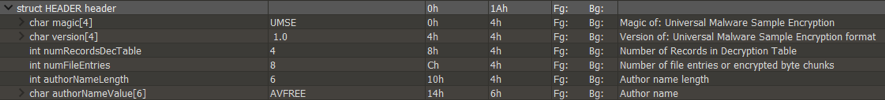
\includegraphics[width=0.99\textwidth]{./figures/UMSEHeader}
\end{figure}

\subsection{Decryption table}

Next, there is the \texttt{Decryption table}. This table contains AES
keys and IVs asociated to each confidentiality level. This keys are used to
encrypt chunks regarding the confidentiality level.  Each table entry contains
an AES key and IV, both wrapped with RSA public key and stored into the
\texttt{aesWrapped} field. And corresponding confidentiality level is stored
into \texttt{levelOfConfidentiality} field.
\begin{figure}[h]
  \centering
  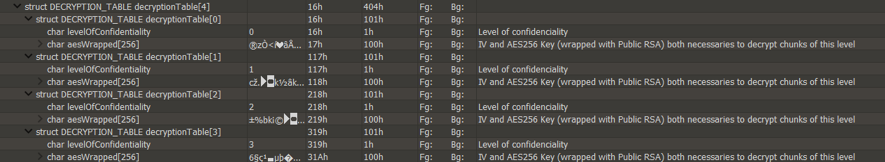
\includegraphics[width=0.99\textwidth]{./figures/UMSEDT}
\end{figure}

\subsection{Entries}

Each sample chunk is stored (encrypted) as an entry regarding its
confidentiality level. Each entry has: a field named \texttt{size} indicating
the size of the encrypted content, a field named
\texttt{levelOfConfidentiality} indicating the chunk encrypted confidentiality
level, a field named \texttt{encryptedMessage} containing the encrypted chunk,
a field named \texttt{numMetadata} indicating the number of metadata entries
associated to the chunk.
\begin{figure}[h]
  \centering
  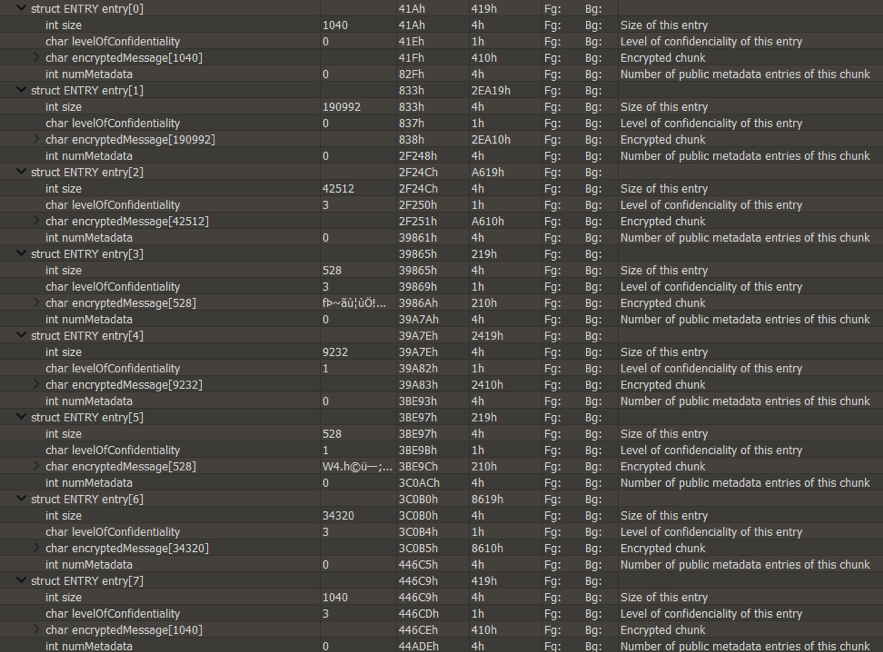
\includegraphics[width=0.99\textwidth]{./figures/UMSEEntries}
\end{figure}

\subsection{File properties}
An additional entry indicating properties which applies to the entire file do
exist.
\begin{figure}[h]
  \centering
  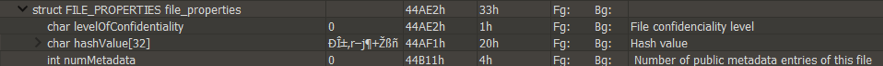
\includegraphics[width=0.99\textwidth]{./figures/UMSEFP}
\end{figure}

\subsection{Authentication header}

Finally, an HMAC checksum of the file is generated. The key used to generate
this HMAC checksum is the SHA256 hash of the RSA decrypted \texttt{decryption
  table}.
\begin{figure}[h]
  \centering
  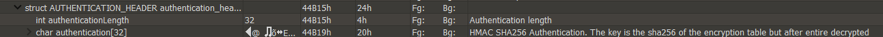
\includegraphics[width=0.99\textwidth]{./figures/UMSEAH}
\end{figure}

Authentication header is absolutely necessary. For instance, an analyst who
has not sufficient privilege to decrypt an UMSE entry, will not be able to
generate another UMSE file with the entry confidentiality level downgraded, in
order to decrypt it.  It protects from padding oracle attacks\cite{Eurocrypt2002}\cite{Oaep} as well. This
block is complementary to encryption.

\subsection{RSA private key}

This is an optional (and generally not recommended) field used to embed the
private RSA key into the file. It can be useful in some cases when
confidentiality is not an issue but the analyst want to exploit the UMSE
format capabilities (see section: 12.5 UMSE tools).
\begin{figure}[h]
  \centering
  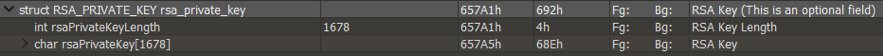
\includegraphics[width=0.99\textwidth]{./figures/UMSEPK}
\end{figure}

\section{UMSE implementation}

\subsection{UMSE C/C++ library}
A C/C++ library was developed to work more easily with UMSE. As most of
security products are developed in C/C++, the UMSE library was developed in
these languages but note that it can be used with independence of the
programming language, for instance, the author integrated it with Python and,
obviously, it worked. The library project follows a standard C project
structure\cite{CanonicalProjectStructure} (see Figure~\ref{fig:UMSELibrary}:
\begin{itemize}
\item \texttt{bin} directory: Compiled resulting binaries are putted inside
  this directory.
\item \texttt{build}: Building files are putted in this directory.
\item \texttt{doc} Documentation directory.
\item \texttt{include}: Includes are here. A subfolder named \texttt{include}
  also exists and it is used to store third party includes.
\item \texttt{lib}: Library files are stored here.
\item \texttt{src}: The program source code.
\item \texttt{test}: Some code to test the library.
\end{itemize}

\begin{figure}
  \centering
  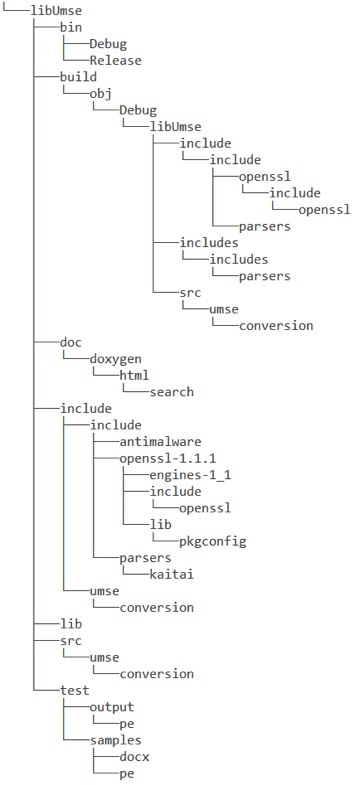
\includegraphics[width=0.5\textwidth]{./figures/UMSELibrary}
  \caption{\label{fig:UMSELibrary} Structure of the UMSE library.}
\end{figure}
\begin{figure}
  \centering
  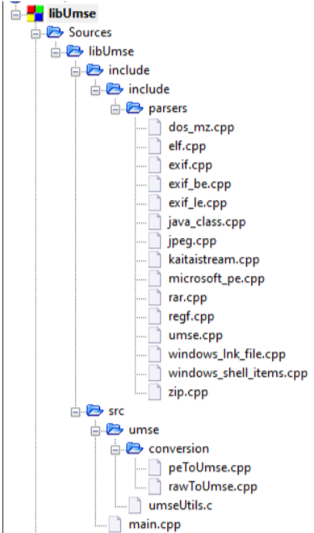
\includegraphics[width=0.5\textwidth]{./figures/UMSEProject}
  \caption{\label{fig:UMSELibrary} Organization of the UMSE project.}
\end{figure}

The project content can be summarized as follows
(Figure~\ref{fig:UMSEProject}):
\begin{itemize}
\item the \texttt{parsers} directory contains a lot of common file type
  parsers for C++. These parsers were generated automatically by Kaitai
  Struct. Parsers folder includes also \texttt{umse.cpp} in order to
  demonstrate that UMSE specification works as expected and it is implemented.
\item the \texttt{conversion} directory implements the conversion from every
  specific file format or chunk structure to UMSE. In file headers of each
  file format/chunk structure converter are defined parameters to calculate
  the corresponding confidentiality level of each file part.
\item the \texttt{umseUtils.c} all necessary functions to deal with UMSE file
  format are developed here. It is not dependent from Kaitai Struct in order
  to allow you to re-use it in other projects.
\item the \texttt{main.cpp} library exported functions are written here and
  some testing/debugging code is also written here.
\end{itemize}

The library exported functions are displayed in
Tables~\ref{fig:f1}-\ref{fig:f3}.
\begin{table}
  \centering
  \begin{tabular}{|l|p{0.7\textwidth}|} \hline
    Description	& This function converts a chunk to Universal Malware Sample
                  Encryption format. \\ \hline
    Input parameters &	\texttt{chunkLength} \\
                     & \texttt{chunk} \\ \hline
    Output parameters & \texttt{umseSize} \\
                      & \texttt{umse} \\ \hline
    Return value & \texttt{void} \\ \hline
    Function header	&
\begin{verbatim}
void DLL_EXPORT ChunkToUmse(
        unsigned int chunkLength,
        unsigned char* chunk,
        unsigned int* umseSize,
        unsigned char** umse
);
\end{verbatim}
    \\ \hline
  \end{tabular}
  \caption{\label{fig:f1} Function f1.}
\end{table}
\begin{table}
  \centering
  \begin{tabular}{|l|p{0.7\textwidth}|} \hline
    Description	& If UMSE integrity check is successful, this function
                  decrypts an entry of a given Universal Malware Sample
                  Encryption file chunk and its RSA Private key.  \\ \hline
    Input parameters &	\texttt{chunkLength} \\
                & \texttt{chunk} \\
                & \texttt{entryToDecrypt} \\
                & \texttt{accessLevel} \\
                & \texttt{rsaPrivateKey} \\ \hline
    Output parameters & \texttt{decryptedEntryLength} \\
                      & \texttt{decryptedEntry} \\ \hline
    Return value & $-2$ if integrity check iss not successful \\
                & $-1$ if \texttt{entryToDecrypt} does not exist \\
    & $0$ if the function ends without errors. \\ \hline
    Function header	&
\begin{verbatim}
int DLL_EXPORT DecryptUmse(
        unsigned int umseLength,
        unsigned char* umse,
        unsigned int entryToDecrypt,
        unsigned int accessLevel,
        char* rsaPrivateKey,
        unsigned int* decryptedEntryLength,
        unsigned char** decryptedEntry
);
\end{verbatim}
    \\ \hline
  \end{tabular}
  \caption{\label{fig:f2} Function f2.}
\end{table}
\begin{table}
  \centering
  \begin{tabular}{|l|p{0.7\textwidth}|} \hline
    Description	& This function checks UMSE integrity.  \\ \hline
    Input parameters &	\texttt{chunkLength} \\
                & \texttt{chunkLength unsigned int} \\
                & \texttt{chunk unsigned char *} \\ \hline
    Output parameters & \texttt{umseSize unsigned int *} \\
                      & \texttt{umse unsigned char **} \\ \hline
    Return value & True if integrity check is successful, otherwise it returns
    false \\ \hline
    Function header	&
\begin{verbatim}
bool DLL_EXPORT CheckUmseIntegrity(
                unsigned int umseLength,
                unsigned char* umse,
                char* rsaPrivateKey
);
\end{verbatim}
    \\ \hline
  \end{tabular}
  \caption{\label{fig:f3} Function f3.}
\end{table}

\section{UMSE agent}

The UMSE Agent is an extremely simple Python program to demonstrate how to
collect system elements, transform it to UMSE, and sent the resulting UMSE
samples to a central intelligence server.
\begin{table}[h]
  \centering
  \begin{tabular}{|l|p{0.55\textwidth}|} \hline
    Files & Purpose \\ \hline
    \texttt{aboutform.py} & A simple form showing information about the
                            program. \\ \hline
    \texttt{av\_agent.py} & PyQt5 System Tray Icon entrypoint. \\ \hline
    \texttt{intelligenceclient.py} & REST API functions for communicating with
                                     UMSE Server. \\ \hline
    \texttt{scanfiles.py} & Element collector, UMSE conversion and sending via
                            \texttt{libUmse.dll}. \\ \hline
    \texttt{trayicon.py} & System Tray Icon implementation. \\ \hline
  \end{tabular}
\end{table}

The agent must to be launched as follows:
\begin{tcolorbox}
  \verb|start /D . C:\Python\Python37\pythonw.exe av_agent.py|
\end{tcolorbox}

\noindent and this is how the agent looks like. Options are self-explanatory
but notice that the \texttt{Collect malware samples} option means collect
samples, convert it to UMSE and automatically send it to the UMSE server.
\begin{figure}[h]
  \centering
  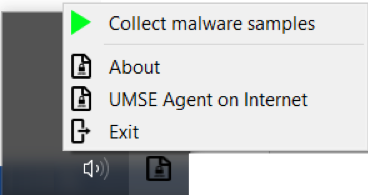
\includegraphics[width=0.4\textwidth]{./figures/UMSEAgent}
\end{figure}

\subsection{UMSE server}

The UMSE server is composed of the following files (see
Figure~\ref{fig:UMSEServer}):
\begin{figure}
  \centering
  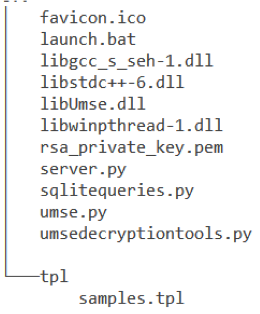
\includegraphics[width=0.4\textwidth]{./figures/UMSEServer}
  \caption{\label{fig:UMSEServer} Structure of the UMSE server.}
\end{figure}

\begin{itemize}
\item \texttt{favicon.ico}: The web application favicon.
\item \texttt{launch.bat}: Simple batch file to start the program.
\item \texttt{libgcc\_s\_sheh-1.dll}, \texttt{libstdc++-6.dll},
  \texttt{libwinpthread-1.dll}: Some \texttt{libUmse.dll} dependencies.
\item \texttt{libUmse.dll}: The compiled UMSE C/C++ library.
\item \texttt{rsa\_private\_key.pem}: RSA Private key which allows UMSE sample
  parts decryption.
\item \texttt{server.py}: A Cherrypy server implementing an extremely simple
  intelligence webpage and REST API to allow the agent to operate with
  samples. Samples are stored in a SQLite database.
\item \texttt{sqlitequeries.py}: SQLite queries are defined here.
\item \texttt{umse.py}: Kaitai Struct UMSE file format parser.
\item \texttt{umsedecryptiontools.py}: Python functions allowing to decrypt an
  UMSE entry (functionality is implemented by \texttt{libUmse.dll}. It is only
  a bridge to it).
\item \texttt{tpl/samples.tpl}: HTML with JAVASCRIPT template used by
  Cherrypy.
\end{itemize}

This is how intelligence panel looks like. It is extremely simple. Only
sample listing (- and + are shortcut keys to go back and forward), sample
search, and sample downloading features are implemented. But note that REST
API requires authentication in order to decrypt samples, and every decryption
operation is logged into SQLite database access logging table.
\begin{figure}[h]
  \centering
  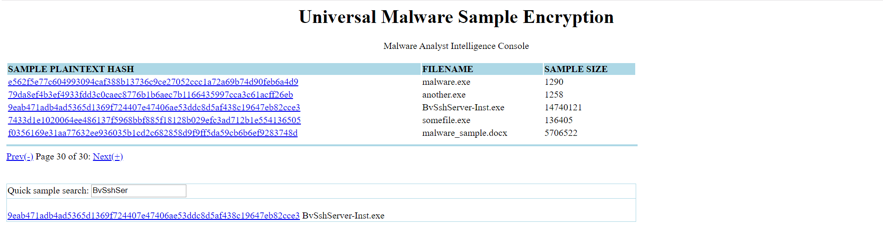
\includegraphics[width=0.99\textwidth]{./figures/UMSEPanel}
  \caption{\label{fig:UMSEPanel} Some caption.}
\end{figure}

\subsection{UMSE Shell}

An extremely simple command line tool implemented in Python which allows you
to interact with the UMSE server. All implementation remains into the
\texttt{umse\_shell.py} file which looks as follows:
\begin{figure}[h]
  \centering
  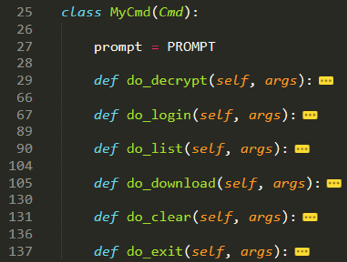
\includegraphics[width=0.4\textwidth]{./figures/UMSEShell}
\end{figure}

\begin{table}[h]
  \centering
  \begin{tabular}{|l|p{0.7\textwidth}|} \hline
    \textsc{Method} & \textsc{Description} \\ \hline
    \texttt{do\_list} &	List samples stored in the UMSE server. \\ \hline
    \texttt{do\_download} & Download samples from the server. \\ \hline
    \texttt{do\_login} & Login into the server. \\ \hline
    \texttt{do\_decrypt} & Decrypt an entry of an UMSE sample (login is
                           required). \\ \hline
    \texttt{do\_clear} & Clear screen. \\ \hline
    \texttt{do\_exit} & Exit the program. \\ \hline
  \end{tabular}
\end{table}

And this is how this console looks like.
\begin{figure}[h]
  \centering
  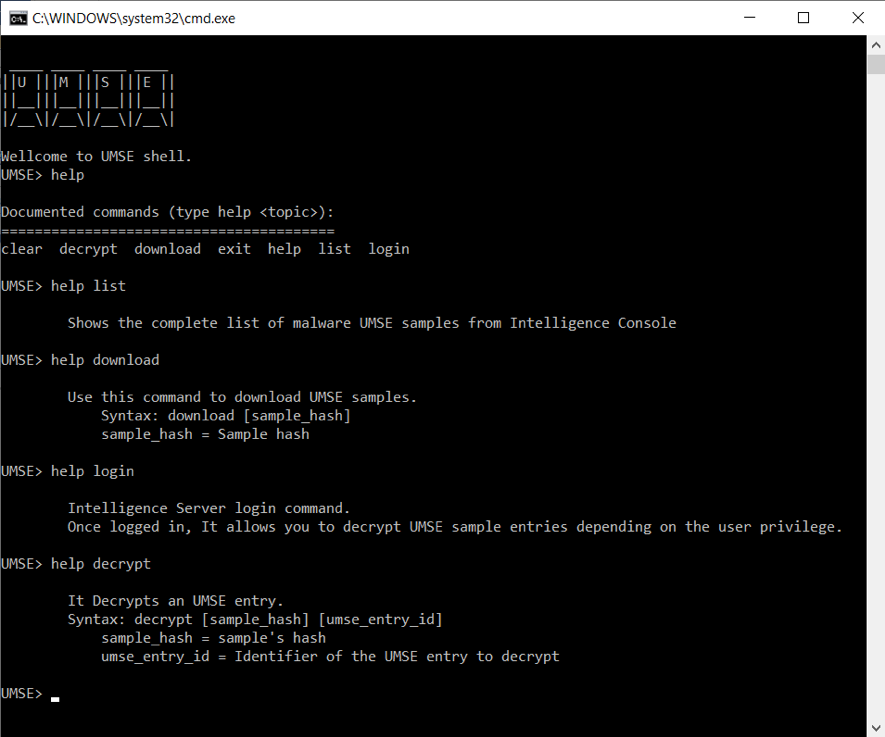
\includegraphics[width=0.95\textwidth]{./figures/UMSEConsole}
\end{figure}

\subsection{UMSE tools}

The UMSE format RSA encryption is a key feature but, in some situations like
when sharing malware between colleagues encryption can be a hindrance. In this
situations you can embed the RSA private key into the sample and don’t care
about encryption anyway.  In this way, the analyst is benefiting himself by
using a specific format to share malware files and, in a future version of
this simple python tool, of metadata and heterogeneous element per sample
appending capabilities of UMSE format.  You can use a simple Python tool
(\texttt{tool\_for\_single\_users.py}) developed for this purpose:
\begin{figure}[h]
  \centering
  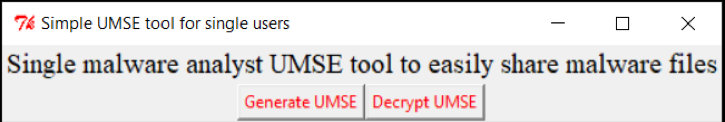
\includegraphics[width=0.75\textwidth]{./figures/UMSETool}
\end{figure}
\chapter{Conclusions and future work}

The UMSE malware sample format improves malware reverse engineering processes\cite{ContextBasedMalware}\cite{LearningFromContext}\cite{ResidentViruses}\cite{FilelessAttacks}\cite{AdvacedVolatileThreat}
and also allows security products (including those which comes built-in the
operating system) to be polite with potentially confidential elements and
information about its clients and users.  Antivirus enterprises do not seem to
be interested in spying the user\cite{BBCMarcinKleczynski}, but maybe they collaborate with a third
party who also uses intelligence information for purposes unrelated to malware
analysis\cite{KasperskyBoundariesOfTrust}. By using UMSE, antivirus products can take the malware sample
treatment control in a transparent way and also protect users' data from a
hypothetical malicious third party.  With the arrival of cyber threat hunting
products (extremely aggressive products against confidentiality), antivirus
comparison tools must take seriously into account the issues of
confidentiality. The rest of features are already sufficiently competed.
Therefore, clients and users must take confidentiality into account while
choosing between them.  It is possible to keep the protection ratio and users
confidentiality at the same time if UMSE is used to acquire, transport and
store the samples.

There of course some developments and features which were not implemented in
UMSE so far. among the possible extensions that the tool could integrate, we
would like to mention the following ideas for future work:
\begin{itemize}
\item UMSE version 1.0 does not specify malware samples metadata. In order to
  be as flexible as possible, it lets this definition absolutely open to
  security tools which implements UMSE. The future work consist in to develop
  a sufficiently general malware UMSE metadata standard to reduce security
  tools UMSE implementation curve.
\item Current UMSE dynamic linking library includes some target format to UMSE
  converters \texttt{xxxToUmse.cpp}. For instance, \texttt{peToUMSE.cpp} was
  developed. We recognize that the mentioned converter file is too simple
  (special cases could lead to errors) and does not take advantage of Portable
  Executable granularity (for instance, it does not encrypt each binary
  resource separately). We let this improvement and the incorporation of new
  converters for a future work.
\item The main purpose of this work is to uncover some shortcomings in the
  current techniques for treating malware samples, and to provide a solution
  to them. Unfortunately, for reasons of time, we could not incorporate this
  mechanism to any existing open source solution for antimalware, like
  Clamav\footnote{\href{https://github.com/Cisco-Talos/clamav-devel}{\texttt{https://github.com/Cisco-Talos/clamav-devel}}}
  for instance, letting it also open for a future work.
\item Improve and add support of metadata and heterogeneous element per sample
  to ``Simple UMSE tool for single users'' mentioned in section XXX.
\end{itemize}
\begin{thebibliography}{0}

  \bibitem{EuropeanParliamentReportOnCyberDefence}
    Paet, U. (25/05/2018). European Parliament: REPORT on cyber defence.
    \url{http://www.europarl.europa.eu/doceo/document/A-8-2018-0189_EN.pdf?redirect}

  \bibitem{EuropeanParliamentDesignatingAsDangerous}
    Annemans, G. (13/06/2018). European Parliament: Designating programmes and companies as 'dangerous' from the point of view of cyber
defence
    \url{http://www.europarl.europa.eu/doceo/document/P-8-2019-001206_EN.pdf}

  \bibitem{Kaspersky2020EulaEn}
    Lab., K. (2019). Kaspersky Lab. Retrieved from Kaspersky Lab.
    \url{https://products.s.kaspersky-labs.com/homeuser/kav2020/20.0.14.1085abc/english-INT-0.2007.0/3231373433327c44454c7c4e554c4c/eula_en.txt}

  \bibitem{McAfeeEnterpriseEulaEnGb}
    McAfee (April, 2018). McAfee. Retrieved from McAfee.
    \url{https://www.mcafee.com/enterprise/en-us/assets/legal/end-user-license-agreements-en-gb.pdf}

  \bibitem{MalwarebytesEula}
    Malwarebytes (2020). Malwarebytes. Retrieved from Malwarebytes:
    \url{https://www.malwarebytes.com/eula/}

  \bibitem{KasperskyBoundariesOfTrust}
    Lab., K. (2019). Kaspersky Lab. Retrieved from Kaspersky Lab. blog:
    \url{https://www.kaspersky.com/blog/the-boundaries-of-trust/}

  \bibitem{ThreatHuntingForDummies}
    Threat Hunting For Dummies® Carbon Black Special Edition. Peter H. Gregory

  \bibitem{ProactiveHunting}
    PROACTIVE HUNTING The Last Line of Defense Against the “Mega Breach”

  \bibitem{HardwareMalware}
    Hardware malware. [S.l.]: Morgan & Claypool. ISBN 9781627052528.

  \bibitem{ContextBasedMalware}
    Analysis and classification of context-based malware behavior. Mohammadhadi Alaeiyan, Saeed Parsa, Mauro Conti

  \bibitem{LearningFromContext}
    Learning from Context: Exploiting and Interpreting File Path Information for Better Malware Detection. Adarsh Kyadige, Ethan M. Rudd, Konstantin Berlin

  \bibitem{SoftwareEngineering}
    Richard F. Schmidt, in Software Engineering, 2013

  \bibitem{ResidentViruses}
    Sharma, S (2013). "Terminate and Stay Resident Viruses" (PDF). International Journal of Research in Information Technology. 1 (11): 201–210.

  \bibitem{FilelessAttacks}
    "Fileless attacks against enterprise networks". Secure List. Secure List. Retrieved 20 February 2017.

  \bibitem{AdvacedVolatileThreat}
    "Advanced volatile threat: New name for old malware technique?". CSO. CSO. Retrieved 20 February 2017.

  \bibitem{MicrosoftPecoff}
    Microsoft Portable Executable and Common Object File Format Specification. Revision 6.0 February 1999. Microsoft Corporation.

  \bibitem{DynamicLinkLibraries}
    Corporation, M. (31/05/2018) Microsoft Corporation. Retrieved from Microsoft Docs.
    \url{https://docs.microsoft.com/es-es/windows/win32/dlls/dynamic-link-libraries?redirectedfrom=MSDN}

  \bibitem{Nist2013}
    NIST (April, 2013). Rebecca M. Blank and Patrick D. Gallagher. Security and Privacy Controls for Federal Information Systems and Organizations. Retrieved from NIST.
    \url{https://nvlpubs.nist.gov/nistpubs/SpecialPublications/NIST.SP.800-53r4.pdf}

  \bibitem{Rfc4949}
    RFC (August, 2007). R. Shirey. Obtained from Internet Engineering Task Force.
    \url{https://tools.ietf.org/html/rfc4949}

  \bibitem{NistGlossary2020}
    NIST (2020). NIST. Retrieved from NIST glossary.
    \url{https://csrc.nist.gov/glossary/term/malware}

  \bibitem{LayeredDetectionMethod}
    A Layered Detection Method for Malware Identification. Ting Liu, Xiaohong Guan, Yu Qu, Yanan Sun

  \bibitem{RussianStoleNsaSpySecrets}
    Lubold, Gordon; Harris, Shane (6 October 2017). "Russian Hackers Stole NSA Spy Secrets". The Wall Street Journal. New York City. pp. 1, 4. Retrieved 12 October 2017

  \bibitem{KasperskyToolForSpying}
    Harris, Shane; Lubold, Gordon (2017-10-11). "Russia Has Turned Kaspersky Software Into Tool for Spying". Wall Street Journal. ISSN 0099-9660. Retrieved 2017-10-19.

  \bibitem{KasperskyTransparencyCenter}
    Lab., K. (2020). Kaspersky Lab. Retrieved from Kaspersky Lab.
    \url{https://www.kaspersky.com/transparency-center}

  \bibitem{EugeneKasperskyBlog2017}
    Kaspersky, E. (30/06/2017). Eugene Kaspersky. Retrieved from Eugene Kaspersky blog.
    \url{https://eugene.kaspersky.com/2017/06/30/keeping-cybersecurity-separate-from-geopolitics/}

  \bibitem{McAfeeEnterpriseEula2019}
    McAfee (June, 2019). McAfee. Retrieved from McAfee.
    \url{https://www.mcafee.com/enterprise/en-us/assets/legal/end-user-license-agreements-en-us.pdf}

  \bibitem{KaitaiStructDoc}
    Struct, K. (2020). Kaitai Struct. Retrieved from Kaitai Struct documentation.
    \url{https://doc.kaitai.io/}

  \bibitem{MalwarebytesUserGuide}
    Malwarebytes for Windows User Guide. Version 3.6.1. 19 September 2018. Copyright © 2018 Malwarebytes. All rights reserved.

  \bibitem{AmazonS3RestApi}
    Amazon (2020). Amazon Web Services, Inc. Retrieved from Amazon S3 documentation.
    \url{https://docs.aws.amazon.com/es_es/AmazonS3/latest/dev/RESTAPI.html}

  \bibitem{MalwarebytesPremium}
    Malwarebytes (2020). Malwarebytes. Retrieved from Malwarebytes.
    \url{https://es.malwarebytes.com/premium/}

  \bibitem{ZeltserShareMalware}
    Zeltser, L. (24/03/2018) Lenny Zeltser. Retrieved from Lenny Zeltser.
    \url{https://zeltser.com/share-malware-with-researchers/}

  \bibitem{MicrosoftDefenderAtp2020}
    Corporation, M. (01/14/2020) Microsoft Corporation. Retrieved from Microsoft Docs.
    \url{https://docs.microsoft.com/en-us/windows/security/threat-protection/microsoft-defender-atp/advanced-hunting-schema-reference}

  \bibitem{CarbonBlack2017}
    CarbonBlack (April, 2017). CarbonBlack. Retrieved from CarbonBlack.
    \url{https://www.carbonblack.com/wp-content/uploads/2017/04/BanHash-B.png}

  \bibitem{MicrosoftRdpCrashes2019}
    Corporation, M. (07/11/2019) Microsoft Corporation. Retrieved from Microsoft blog site.
    \url{https://www.microsoft.com/security/blog/2019/11/07/the-new-cve-2019-0708-rdp-exploit-attacks-explained/}

  \bibitem{VirusTotalFileSearch2020}
    VirusTotal (2020). VirusTotal. Retrieved from VirusTotal file search:
\url{https://www.virustotal.com/intelligence/help/file-search/}

  \bibitem{IntrusionDetectionNetworks}
    Intrusion Detection Networks: A Key to Collaborative Security. Carol Fung, Raouf Boutaba

  \bibitem{AVComparatives2020}
    AV-Comparatives (2020). AV-Comparatives. Retrieved from AV-Comparatives:
    \url{https://www.av-comparatives.org/}

  \bibitem{AVTest}
    AV-Test (2020). AV-Test. Retrieved from AV-Test.
    \url{https://www.av-test.org/}

  \bibitem{AVComparativesResults2019}
    AV-Comparatives (July, 2019). AV-Comparatives. Retrieved from AV-Comparatives.
    \url{https://www.av-comparatives.org/tests/business-security-test-2019-march-june/}

  \bibitem{VXVault2020}
    VXVault (2020). VXVault. Retrieved from VXVault.
    \url{http://vxvault.net/ViriList.php}

  \bibitem{VirusTotalUpload2020}
    VirusTotal (2020). VirusBay. Retrieved from VirusTotal.
    \url{https://www.virustotal.com/gui/home/upload}

  \bibitem{MalShare2020}
    MalShare (2020). MalShare. Retrieved from MalShare.
    \url{https://malshare.com/}

  \bibitem{VirusShare2020}
    VirusShare (2020). VirusShare. Retrieved from VirusShare.
    \url{https://virusshare.com/}

  \bibitem{VirusBay2020}
    VirusBay (2020). VirusBay. Retrieved from VirusBay.
    \url{https://beta.virusbay.io/sample/browse}

  \bibitem{VirusTotalTermsOfService2020}
    VirusTotal (2020). VirusTotal. Retrieved from VirusTotal Terms of Service.
    \url{https://support.virustotal.com/hc/en-us/articles/115002145529-Terms-of-Service}

  \bibitem{NistGlossaryFirmware2020}
    NIST (2020). NIST. Retrieved from NIST glossary.
    \url{https://csrc.nist.gov/glossary/term/firmware}

  \bibitem{AuthenticatedEncryption2000}
    Bellare M., Namprempre C. (2000) Authenticated Encryption: Relations among Notions and Analysis of the Generic Composition Paradigm. In: Okamoto T. (eds) Advances in Cryptology — ASIACRYPT 2000. ASIACRYPT 2000. Lecture Notes in Computer Science, vol 1976. Springer, Berlin, Heidelberg

  \bibitem{Eurocrypt2002}
    Serge Vaudenay (2002). Security Flaws Induced by CBC Padding Applications to SSL, IPSEC, WTLS... EUROCRYPT 2002.

  \bibitem{Oaep}
    Manger, James. "A Chosen Ciphertext Attack on RSA Optimal Asymmetric Encryption Padding (OAEP) as Standardized in PKCS #1 v2.0". Telstra Research Laboratories.

  \bibitem{AuthenticatedEncryption2013}
    "Information technology -- Security techniques -- Authenticated encryption". 19772:2009. ISO/IEC. Retrieved March 12, 2013.

  \bibitem{CanonicalProjectStructure}
    Canonical Project Structure. Boris Kolpackov 2018-10-08

  \bibitem{ClamAV}
    ClamAV (2020). ClamAV. Retrieved from ClamAV Github site.
    \url{https://github.com/Cisco-Talos/clamav-devel}

  \bibitem{BBCMarcinKleczynski}
    BBC (22/07/2019). Joe Tidy. Retrieved from BBC News.
    \url{https://www.bbc.com/news/business-49015609}


\end{thebibliography}

%\appendix
%\chapter{Dummy Appendix}

You can defer lengthy calculations that would otherwise only interrupt
the flow of your thesis to an appendix.


\backmatter

\bibliographystyle{plain}
\bibliography{refs}

%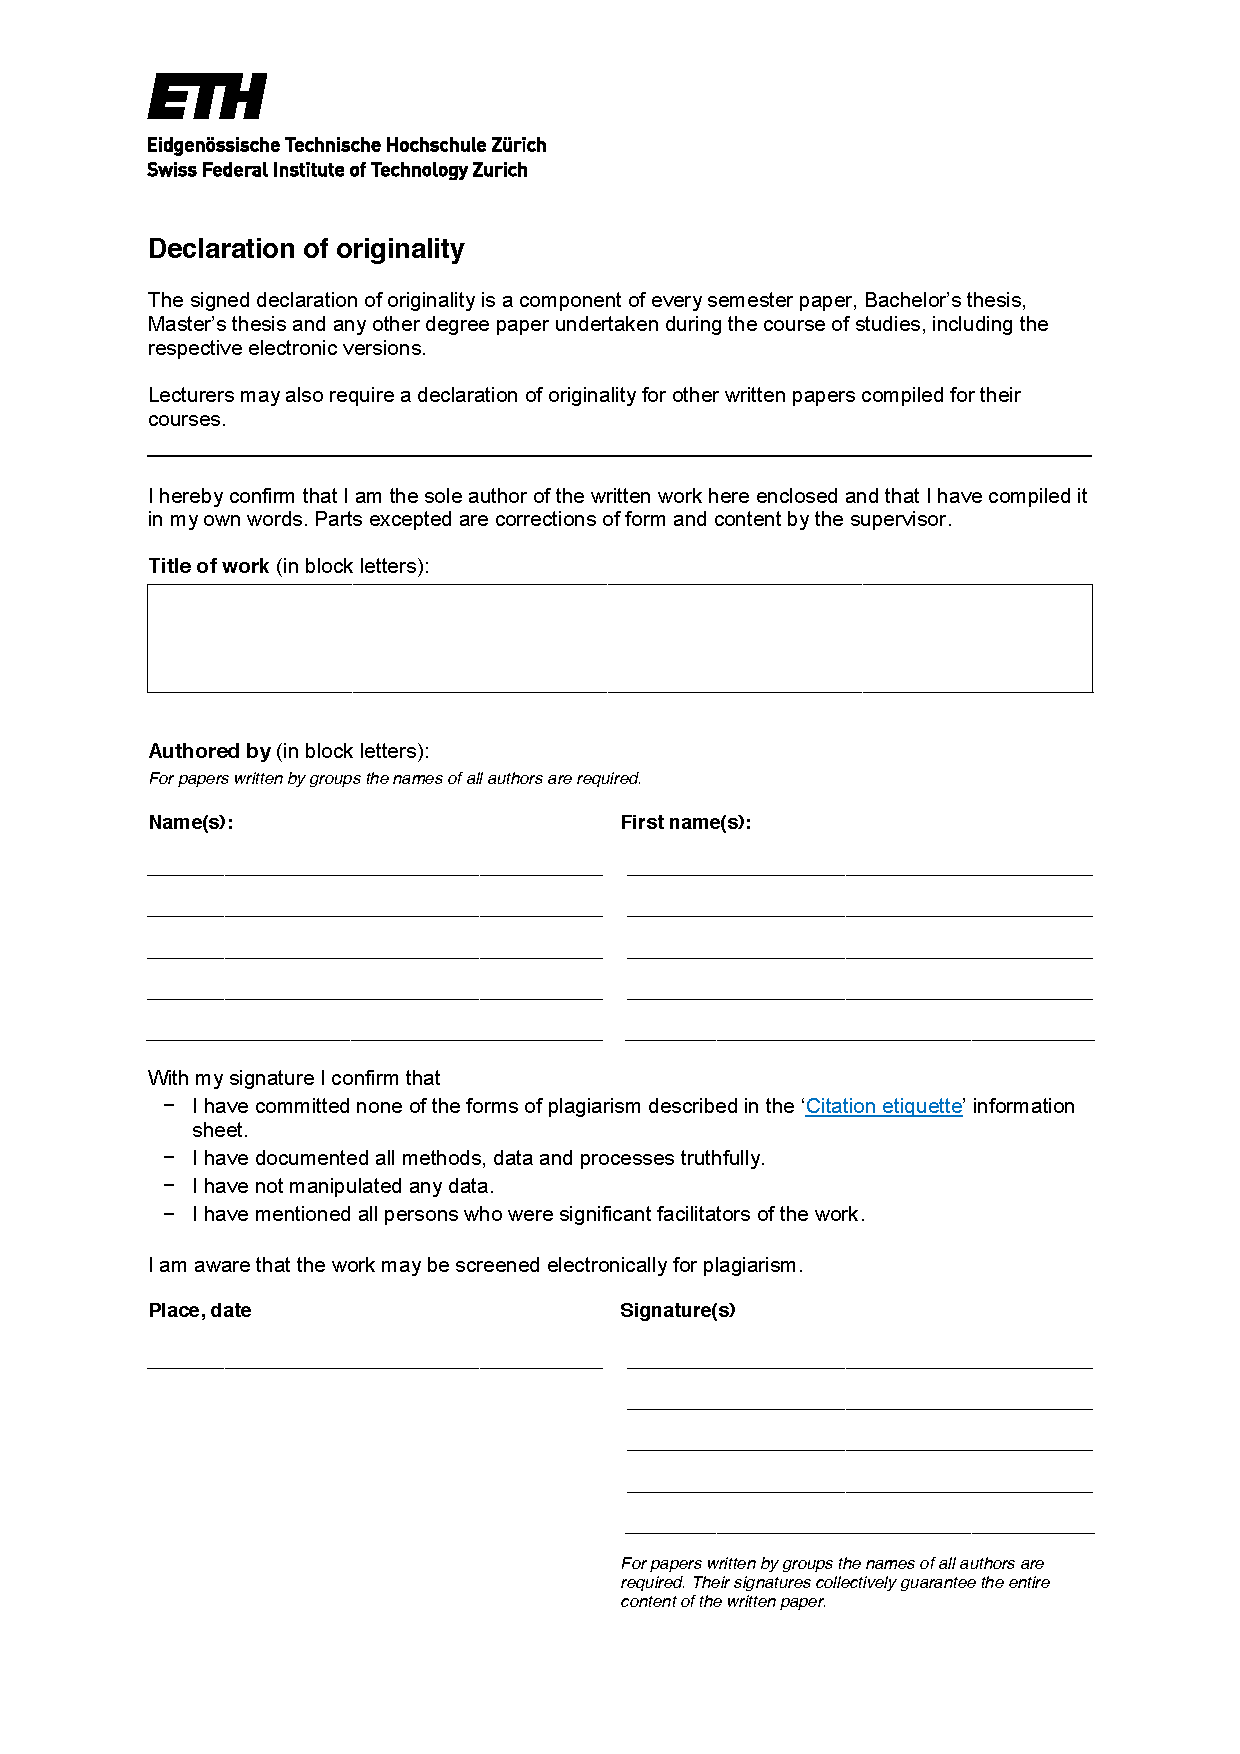
\includepdf[pages={-}]{declaration-originality.pdf}

\end{document}
